\documentclass[10pt]{article}
\usepackage[utf8]{inputenc}
\usepackage[margin=1in]{geometry}
\usepackage{setspace}
\usepackage{color,xcolor}
\usepackage{float}
% \usepackage[subrefformat=parens,labelformat=parens]{subfig}
\usepackage[subrefformat=parens,labelformat=parens]{subcaption}
\usepackage{natbib}
\usepackage{booktabs}
\usepackage{tikz}
\usepackage{multirow}
\usepackage{amsfonts}
\usepackage{amsmath}
\usepackage{amsthm}
\usepackage{bm}
\usepackage{enumerate}
\usepackage[inline]{enumitem}

\usetikzlibrary{positioning}
\usetikzlibrary{arrows.meta, matrix}
\usetikzlibrary{shapes,arrows,chains}
\usetikzlibrary{arrows,positioning,calc,topaths}

% \usepackage[compact]{titlesec}
\usepackage{titlesec}
\titleformat*{\section}{\large\bfseries}
\titleformat*{\subsection}{\normalsize\bfseries}
\titleformat{\subsubsection}[runin]
  {\normalfont\normalsize\bfseries}{\thesubsubsection}{1em}{}
\titleformat*{\paragraph}{\normalsize\bfseries}
\titleformat*{\subparagraph}{\normalsize\bfseries}


\usepackage[nokeyprefix]{refstyle}
\usepackage{varioref}
\usepackage{xr-hyper}
\RequirePackage[citecolor=blue,colorlinks=true,linkcolor=blue]{hyperref}
\usepackage[capitalise,noabbrev]{cleveref}
\crefformat{equation}{(#2#1#3)}


\theoremstyle{definition}
%\newtheorem{lemma}{Lemma}
\newtheorem{proposition}{Proposition}
\newtheorem{cor}{Corollary}
%\newtheorem{definition}{Definition}
\newtheorem{assumption}{Assumption}
\newtheorem{remark}{Remark}

\newcommand{\commentG}[1]{{\color{purple} \noindent [GP: #1]}}
\newcommand{\E}{\mathbb{E}}
\newcommand{\Var}{\mathrm{Var}}
\newcommand{\indep}{\perp \!\!\! \perp}
\newcommand\numberthis{\addtocounter{equation}{1}\tag{\theequation}}

\setstretch{1.45}

\title{%Causal inference in the presence of unmeasured confounding and interference \\
Spatial causal inference in the presence of unmeasured confounding and interference
%OR\\
%Causal inference with spatial dependencies
}
\author{Georgia Papadogeorgou\thanks{This material is based upon work supported by the National Science Foundation under Grant No. 2124124.} \\
{\normalsize Department of Statistics, University of Florida} \\
and \\
Srijata Samanta \\
{\normalsize Department of Biostatistics, The University of Texas M.D. Anderson Cancer Center.}}
\date{}

\allowdisplaybreaks
\begin{document}

\maketitle

\begin{abstract}
Causal inference in spatial settings is met with unique challenges and opportunities. On one hand, a unit’s outcome can be affected by the exposure at many locations, leading to interference. On the other hand, unmeasured spatial variables can confound the effect of interest. 
Our work has two overarching goals.
First, using causal diagrams, we illustrate that spatial confounding and interference can manifest as each other, meaning that investigating the presence of one can lead to wrongful conclusions in the presence of the other, and that statistical dependencies in the exposure variable can render standard analyses invalid. This can have crucial implications for analyzing data with spatial or other dependencies, and for understanding the effect of interventions on dependent units. 
Secondly, we propose a parametric approach to mitigate bias from local and neighborhood unmeasured spatial confounding and account for interference simultaneously. This approach is based on simultaneous modeling of the exposure and the outcome while accounting for the presence of spatially-structured unmeasured predictors of both variables. We illustrate our approach with a simulation study and with an analysis of the local and interference effects of sulfur dioxide emissions from power plants on cardiovascular mortality.
\end{abstract}

\section{Introduction}

Many of the questions researchers are faced with are causal in nature, and methodology for drawing causal inferences from observational data has been flourishing in the past decades. Most of the methods and theory assume that the available data form a random sample of independent observations from a superpopulation of interest. However, in many contexts, data are not independent, and causal and statistical dependencies complicate both how causal effects are defined and how they are estimated.
Our focus is causal inference with spatial data, though our work readily extends to other structural dependencies such as network settings. When faced with spatial observational data, the data's inherent dependence structure offers unique challenges and opportunities.

One of the challenges pertains to the potential existence of spatial spillover effects: the outcome in one location might be driven by exposures in the same location, but also other locations nearby. This phenomenon is often referred to in the causal inference literature as {\it interference}. When interference is present, causal estimators that ignore it might return quantities that are not interpretable without additional assumptions \citep{Tchetgen2012,savje2021average}.
Interference has attracted a lot of attention in the last couple of decades \citep[e.g.][among many others]{Sobel2006, Hudgens2008, manski2013identification, aronow2017estimating} with some studies that focus explicitly on how interference manifests in spatial settings \citep{Verbitsky-savitz2012, wang2020design, zigler2020bipartite, antonelli2020heterogeneous, papadogeorgou2022causal, giffin2022generalized}.

Spatial data also present opportunities for causal inference that pertain specifically to their dependence structure. One causal assumption often employed to identify causal effects from observational data is that of no unmeasured confounding. If this assumption is not satisfied using only measured covariates, estimated quantities will lack a causal interpretation. If the unmeasured confounders are spatially varying in that nearby observations have similar values, recent developments have harvested this structure to mitigate bias from these unmeasured spatial confounders \citep{thaden2018structural, papadogeorgou2019adjusting, keller2020selecting, schnell2020mitigating, dupont2022spatial, christiansen2022toward, Guan2022spectral}. Therefore, the data's inherent dependence structure provides opportunities to relax the no-unmeasured confounding assumption.

In this work, we investigate the complications that arise when data are inherently dependent, and the co-existence of unmeasured confounding and interference in spatial settings, and propose an approach that aims to control for both.
First, we introduce causal diagrams for spatial data with inherent statistical dependencies.
Second, we illustrate theoretically and practically that spatial confounding and spatial spillover effects can manifest as one another. If unmeasured spatial confounding is present and not accounted, investigators might misinterpret the spatial structures induced by the confounder as interference, which would lead to wrongful conclusions about the causal effect of a potential intervention. In reverse, if interference is present and not accounted, researchers might mis-attribute spatial dependencies induced by interference to spatial confounding. 
Thirdly, we demonstrate that spatial dependencies in the exposure variable can render standard analyses for estimating causal effects invalid, implying unique challenges in the presence of spatial data compared to settings with independent observations.
Fourthly, we suggest an approach that allows us to address unmeasured spatial confounding and interference simultaneously. Specifically, we introduce a set of assumptions under which confounding by unmeasured spatial variables and interference can be accommodated within one unifying context. 
Lastly, we analyze county-level data on the relationship between sulfur dioxide (SO$_2$) emissions from power plants and cardiovascular mortality. The approach that does not account for unmeasured confounding indicates a counter-intuitive protective effect of higher SO$_2$ emissions on health, whereas our approach returns substantively different conclusions that are more in-line with the current knowledge.
Even though we present our findings and conclusions in the context of areal data, extensions to point-referenced spatial data are readily available with appropriate adjustments.


\subsection{Related literature}

The term spatial confounding has been used to represent drastically different notions in the spatial and causal literatures \citep{reich2021review, Gilbert2021approaches, papadogeorgou2022discussion}. Popularized in spatial statistics, spatial confounding was first used to describe collinearity between covariates and spatial random effects in regression models \citep{reich2006effects, Hodges2010, Paciorek2010, Hanks2015, Prates2019alleviating}. Here, we adopt the notion of spatial confounding encountered in causal inference \citep{papadogeorgou2019adjusting, Gilbert2021approaches}, where the measured variables do not suffice for confounding adjustment, but the missing confounders exhibit a spatial structure.

Even though unmeasured spatial confounding and spatial interference have been investigated previously, to our knowledge, there exists limited work that addresses both of these issues simultaneously. In a study of area deprivation on pedestrian casualties, \cite{graham2013quantifying} adopted a modeling approach to spatial confounding and interference which included spatial predictors, spatial random effects, and functions of the neighboring areas' exposure in a Poisson regression. However, their approach does not explicitly clarify the causal quantities of interest, and is susceptible to errors in fixed effects introduced by using spatial random effects \citep{Hodges2010}.
Within a causal inference framework, \cite{giffin2021instrumental} investigated an instrumental-variable approach in the case of spatial data, and they allowed for the effect of the exposure at other locations to affect the outcome. Their approach provides a promising direction forward, though it requires access to a valid instrument.

Particularly relevant is the work by \cite{ogburn2014causal} where they introduced causal diagrams for causal inference with interference, and use these graphs to determine identifiability of causal estimands. They find that neighbors' covariate values often need to be controlled for in order to block all back-door paths. This observation was also established by \cite{forastiere2021identification}, and \cite{tec2022weather2vec} developed an approach using neural networks for finding the appropriate form of the neighborhood covariates. However, the work by \cite{ogburn2014causal} does not directly address non-causal dependencies among observations that might naturally occur in spatial settings. Relatedly, \cite{vansteelandt2007confounding} considers the setting where treatments within a cluster can be correlated due to unmeasured cluster-level variables, but they do not investigate the interplay between statistical dependencies in confounders and exposures.
\cite{rosenbaum2007interference} states that ``Interference is distinct from statistical dependence produced by pretreatment clustering, although both may be present.'' 
Here, we address multiple types of spatial dependencies: spatial interference, spatial dependence occurring due to pre-treatment unmeasured confounders, and inherent spatial co-dependencies.


% \section{Paired spatial data: Estimands and identifiability of local and interference effects in the presence of confounding and spatial dependencies}
\section{Estimands and identifiability of causal effects with paired spatial data}
\label{sec:pairs}

First, we focus on the setting where the population of interest is a collection of blocks of spatial data, where dependencies manifest within a block but not across them. This situation can be a reasonable approximation in situations where dependencies occur in small geographical distances, and available data include regions that are far from each other. For simplicity, we focus on blocks of size two (pairs) though everything readily extents to larger blocks, or blocks of varying sizes, which we discuss briefly in \cref{subsec:blocks_larger}.

\subsection{Causal estimands for paired spatial data with a binary treatment}

We first consider the situation where there is a natural ordering within pairs that allows us to name one unit as Unit 1 and the other as Unit 2. We use $i,j$ to denote the two units, and we drop the notation that corresponds to the block for simplicity. The units are assumed to have potential outcomes $Y_i(z_i, z_j)$ and $Y_j(z_j, z_i)$ for treatments $z_i, z_j \in \{0, 1\}$, where we always write the individual's own treatment first.

We use $\lambda$ to denote {\it local} effects representing the effect on a unit's outcome for changes in its own treatment, and $\iota$ to denote {\it interference} effects representing the effect on a unit's outcome for changes in the neighbor's treatment. Define the local effect for unit $i$ as
\begin{equation}
\begin{aligned}
\lambda_i(0) &= \E[Y_i(z_i = 1, z_j = 0) - Y_i(z_i = 0, z_j= 0)] \equiv \E[ Y_i(1, 0) - Y_i(0, 0)],
\quad \text{and}\\
\lambda_i(1) &= \E[Y_i(z_i = 1, z_j = 1) - Y_i(z_i = 0, z_j= 1)] \equiv \E[ Y_i(1, 1) - Y_i(0, 1)],
\end{aligned}
\label{eq:local_effect}
\end{equation}
and the interference effects for unit $i$ as
\begin{equation}
\begin{aligned}
\iota_i(0) &= \E[Y_i(z_i = 0, z_j = 1) - Y_i(z_i = 0, z_j= 0)] \equiv \E[Y_i(0, 1) - Y_i(0, 0)],
\quad \text{and}\\
\iota_i(1) &= \E[Y_i(z_i = 1, z_j = 1) - Y_i(z_i = 1, z_j= 0)] \equiv \E[Y_i(1, 1) - Y_i(1, 0)],
\end{aligned}
\label{eq:interference_effect}
\end{equation}
where the expectations are over the blocks. Therefore, in the definition of $\lambda_i(z)$ and $\iota_i(z)$, the subscript $i$ represents the unit on whose outcome we focus. Instead, the argument $z$ represents the level at which we fix the neighbor's treatment or the unit's own treatment for the local and interference effects, respectively.

Alternate definitions of local effects draw the treatments for other units from a pre-specified distribution. For $\pi \in [0, 1]$, we use $\lambda_i(\pi)$ to denote the local effect for unit $i$ when the treatment of unit $j$ is drawn from a Bernoulli distribution with probability $\pi$. It holds that $\lambda_i(\pi) = \pi \lambda_i(1) + (1 - \pi) \lambda_i(0)$. Similarly, the interference effect of unit $i$ when their own treatment is drawn from a Bernoulli$(\pi)$ distribution is denoted by $\iota_i(\pi)$ and $\iota_i(\pi) = \pi \iota_i(1) + (1 - \pi) \iota_i(0)$. For $\pi \in \{0, 1\}$ these definitions revert back those in \cref{eq:local_effect} and \cref{eq:interference_effect}.

If there does not exist a natural ordering of the units within a block, then the local and interference causal effects could be defined as
\( \displaystyle
\lambda(z) = \left( \lambda_1(z) + \lambda_2(z) \right) / 2 \), and
$\iota(z) = \left(\iota_1(z) + \iota_2(z) \right) / 2$, respectively, for $z \in \{0, 1\}$.



\subsection{Spatial statistical and causal dependence through a graph lens}


Here, we use graphs to discuss identifiability of the local and interference effects in paired spatial data. Causal graphs have been used to establish identifiability of causal estimands in a variety of settings \citep{pearl2000models} and in the presence of interference explicitly \citep{ogburn2014causal}. Here, we establish causal diagrams in scenarios where spatial confounding and interference might exist separately or simultaneously, and where the treatment itself exhibits spatial statistical dependence. Here, the term {\it spatial interference} is used to represent the situation where the treatment applied in one location affects the outcome in the other location. The term {\it spatial confounding} is used to represent the situation where a spatial variable confounds the relationship of interest, in that it leads to open back-door paths from the treatment to the outcome of interest \citep{pearl1995causal}. The treatment variable is allowed to exhibit correlation across locations, and the value at one location is {\it not causally} driven by the value in other locations.

Our focus is in identifying the complications that spatial structure of different variables can induce in terms of confounding and interference, and also illustrate that spatial confounding can manifest as interference and vice versa.

Let $\bm Z = (Z_1, Z_2)$ and $\bm Y = (Y_1, Y_2)$ denote the block-level observed treatment and outcome for the two units. We assume that the observed outcomes are equal to the potential outcomes under the observed treatment, $Y_1 = Y_1(Z_1, Z_2)$ and $Y_2 = Y_2(Z_2, Z_1)$, and that ignorability holds conditional on a covariate $\bm U= (U_1, U_2)$. 
We denote the covariate with the letter ``U'' since we will think of this covariate as unmeasured later in the manuscript. Additional (measured) covariates could be easily incorporated here, though we avoid doing so for simplicity of our drawn graphs below. 
\begin{assumption}[Paired data ignorability]
It holds that $\bm Z \indep Y_i(z_1, z_2) \mid \bm U$ for $i = 1, 2$ and $z_1, z_2\in \{0, 1\}$.
Also, for each $\bm u = (u_1, u_2)$ such that $P_{\bm U}(\bm u) > 0$, we have that $P_{\bm Z}(\bm z \mid \bm U = \bm u) > 0$, where $\bm z = (z_1, z_2) \in \{0, 1\}^2.$ 
%where $P_{\bm U}$ denotes the distribution of $\bm U$, and $P_{\bm Z}(\cdot \mid \bm U = \bm u)$ denotes the distribution of $\bm Z$ conditional on $\bm U = \bm u$.
\label{ass:paired_ignorability}
\end{assumption}

\cref{fig:dag_compact} depicts the directed acyclic graph (DAG) for the covariate, treatment, and outcome at the block level. An arrow between two variables represents that the variable on the tail of the arrow has an effect on the variable at the head of the arrow. 
The graphical model associated with this DAG would specify that the block-level data have joint density $f(\bm u, \bm z, \bm y) = f(\bm u) f(\bm z \mid \bm u) f(\bm y \mid \bm z, \bm u)$.
Therefore, this graph compacts the variables across the two units in the block which masks the underlying dependencies that are important for investigating identifiability of causal contrasts in different scenarios.

In \cref{fig:dag_expanded} we use a chain graph to depict the two units within the block separately. We use an undirected edge to represent statistical dependence of the random variables on either side. We formally discuss the interpretation of an undirected edge below. Absence of an arrow or edge forces that the corresponding relationship is not present, whereas the presence of an arrow or edge does not necessarily mean that the depicted relationship takes place. The scenarios we consider in this manuscript are depicted in \cref{fig:dag_expanded_considered}. Specifically, we do not delve into the situation where the outcome is inherently spatial ($Y_1, Y_2$ edge missing). We also ignore the case where $U$ in one location predicts $Z$ in a different location, which would increase the number of scenarios to consider without providing many additional insights.
%Therefore, we consider the situation where the treatment assignment is driven by covariates only in the same location.

\begin{figure}[!t]
\vspace{-30pt}
\centering
\begin{subfigure}[t]{.49\linewidth}
\centering
\begin{tikzpicture}
\node (1) {$\bm U$};
\node[right=of 1] (2) {$\bm Z$};
\node[right=of 2] (3) {$\bm Y$};
\draw[->] (1) to (2);
\draw[->] (1) to [out=30,in=150] (3);
\draw[->] (2) to (3);
\phantom{\draw[->] (1) to [out=315,in=315,looseness=2] (3);}
\phantom{\draw[->] (3) to [out=45,in=135,looseness=2] (1);}
\end{tikzpicture}
\vspace{-10pt}
\caption{Compact graph at the block level.}
\label{fig:dag_compact}
\end{subfigure}
\hspace{-50pt}
\begin{subfigure}[t]{.49\linewidth}
\centering
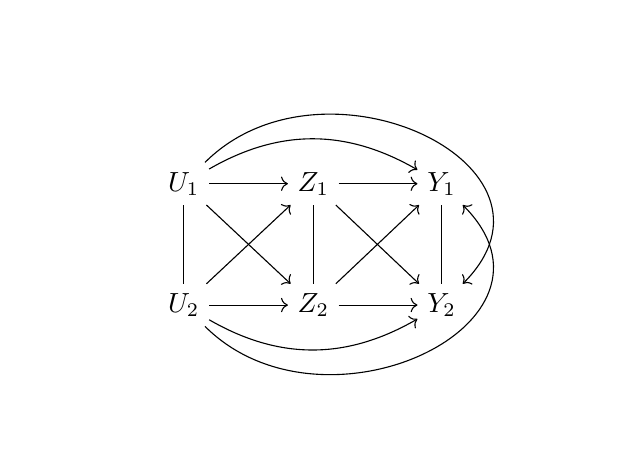
\begin{tikzpicture}
        \node (1) {$U_1$};
		\node[ right= of 1] (2) {$Z_1$};
		\node[ right= of 2] (3) {$Y_1$};
		\node[below = of 1] (12) {$U_2$};
		\node[ right= of 12] (22) {$Z_2$};
		\node[ right= of 22] (32) {$Y_2$};
		\draw[->] (1) to (2); 
		\draw[->] (12) to (2); 
		\draw[->] (1) to (22); 
		\draw[->] (12) to (22); 
		\draw[->] (2) to (3); 
		\draw[->] (2) to (32);
		\draw[->] (22) to (3);
		\draw[->] (12) to [out=330,in=210] (32);
		\draw[->] (1) to [out=45,in=45,looseness=1.5] (32);
\phantom{\draw[->] (32) to [out=45,in=135,looseness=1.5] (1);}
		\draw[->] (12) to [out=315,in=315,looseness=1.5] (3);
		\draw[->] (1) to [out=30,in=150] (3);
		\draw[->] (22) to (32);
		\draw[-] (1) to (12);
		\draw[-] (2) to (22);
		\draw[-] (3) to (32);
\phantom{\node [below left =0.6 and 0.6 of 1] (10) {$U$};}
	\end{tikzpicture}
\vspace{-10pt}
\caption{Two units depicted separately.}
\label{fig:dag_expanded}
\end{subfigure}
%
\begin{subfigure}[t]{.49\linewidth}
\centering
\begin{tikzpicture}
        \node (1) {$U_1$};
		\node[ right= of 1] (2) {$Z_1$};
		\node[ right= of 2] (3) {$Y_1$};
		\node[below = of 1] (12) {$U_2$};
		\node[ right= of 12] (22) {$Z_2$};
		\node[ right= of 22] (32) {$Y_2$};
		\draw[->] (1) to (2); 
		\draw[->] (12) to (22); 
		\draw[->] (2) to (3); 
		\draw[->] (2) to (32);
		\draw[->] (22) to (3);
		\draw[->] (12) to [out=330,in=210] (32);
		\draw[->] (1) to [out=45,in=45,looseness=1.5] (32);
\phantom{\draw[->] (32) to [out=45,in=135,looseness=1.5] (1);}
		\draw[->] (12) to [out=315,in=315,looseness=1.5] (3);
		\draw[->] (1) to [out=30,in=150] (3);
		\draw[->] (22) to (32);
		\draw[-] (1) to (12);
		\draw[-] (2) to (22);
	\end{tikzpicture}
\vspace{-10pt}
\caption{Relationships we consider in this manuscript.}
\label{fig:dag_expanded_considered}
\end{subfigure}
%
\begin{subfigure}[t]{.49\linewidth}
\centering
\begin{tikzpicture}
        \node (1) {$U_1$};
        \node [below left =0.3 and 0.3 of 1] (10) {$U^u$};
        \node [below left =0.3 and 0.3 of 2] (20) {$Z^u$};
		\node[ right= of 1] (2) {$Z_1$};
		\node[ right= of 2] (3) {$Y_1$};
		\node[below = of 1] (12) {$U_2$};
		\node[ right= of 12] (22) {$Z_2$};
		\node[ right= of 22] (32) {$Y_2$};
		\draw[->] (1) to (2); 
		\draw[->] (12) to (22); 
		\draw[->] (2) to (3); 
		\draw[->] (2) to (32);
		\draw[->] (22) to (3);
		\draw[->] (12) to [out=330,in=210] (32);
		\draw[->] (1) to [out=45,in=45,looseness=1.5] (32);
\phantom{\draw[->] (32) to [out=45,in=135,looseness=1.5] (1);}
		\draw[->] (12) to [out=315,in=315,looseness=1.5] (3);
		\draw[->] (1) to [out=30,in=150] (3);
		\draw[->] (22) to (32);
		\draw[->] (10) to (1);
		\draw[->] (10) to (12); 
		\draw[->] (20) to (2);
		\draw[->] (20) to (22);
\end{tikzpicture}
\vspace{-10pt}
\caption{Statistical dependencies occur due to a common underlying structure which is \textit{unobservable}.}
\label{fig:dag_underlying}
\end{subfigure}
\caption{Causal dependencies at the block level. (a) Compacted across units. The covariate $\bm U$ blocks the back-door path from the block-level exposure $\bm Z$ to the block-level outcome $\bm Y$. (b) Units depicted separately, with all possible relationships allowed. Edges denote statistical dependence. (c) Subgraph we consider in this manuscript with some arrows and edges missing. (d) Statistical dependencies are conceived as occurring due an underlying common predictor. This predictor is \textit{unobservable}, in that it can never be measured. }
\label{fig:dag}
\end{figure}

In all the graphs we consider, we allow for spatial dependence within $\bm U$ and within $\bm Z$, depicted with edges between $U_1, U_2$ and between $Z_1, Z_2$. Therefore, the exposure $\bm Z$ is spatial because the spatial variable $\bm U$ is a predictor of $\bm Z$ (illustrated through $Z_1 \leftarrow U_1 - U_2 \rightarrow Z_2$), and because $\bm Z$ is inherently spatially structured (illustrated through the direct connection $Z_1 - Z_2$). Chain graphs can have different causal interpretations \citep{lauritzen2002chain}. Here, we consider undirected edges as representing inherent statistical dependencies due to a common underlying spatial trend. A DAG that would represent this structure is shown in \cref{fig:dag_underlying}. Here, $U^u$ induces correlation between $U_1$ and $U_2$, and similarly for $Z^u, Z_1$, and $Z_2.$ Therefore, the graphical model associated with the chain graph in \cref{fig:dag_expanded_considered} is the graphical model for the DAG in \cref{fig:dag_underlying}, and can be written as
\begin{equation}
\begin{aligned}
f& (u^u, \bm u, z^u, \bm z, \bm y) = \\
&= f(u^u) f(u_1 \mid u^u) f(u_2 \mid u^u) f(z^u) f(z_1 \mid z^u, u_1) f(z_2 \mid z^u, z_2) f(y_1 \mid z_1, z_2, u_1, u_2) f(y_2 \mid z_2, z_1, u_2, u_1)
\end{aligned}
\label{eq:graphical_model}
\end{equation}
The superscript $^u$ is used to stand for Underlying, Unobservable variables that drive the spatial structure in the corresponding variable.
We stress here that the statistical dependencies in the chain graph of \cref{fig:dag_expanded_considered} are crucially different than conceiving the underlying $U^u$ and $Z^u$ in \cref{fig:dag_underlying} as unmeasured variables. 
For example, let's assume that $\bm U = (U_1, U_2)$ is drawn from a bivariate normal distribution with variances equal to 1 and correlation parameter $\rho$. Generating $\bm U$ in this way is equivalent to drawing $U^u, \epsilon_1, \epsilon_2$ independently from $N(0, 1)$ and setting $U_i = \rho U^u + (1 - \rho)\epsilon_i$, $i = 1, 2$. Here $U^u$ would represent the common trend between the $U_i$s, but $U^u$ does not ``exist.'' Therefore, even though $U^u$ can be conceived to {\it drive} the underlying common trend in $(U_1, U_2)$, $U^u$ and $Z^u$ are truly unobserv\textit{able}, they can {\it never} be measured directly, they cannot be directly conditioned on, and therefore should {\it not} be thought of as missing confounding variables. Lastly, since $U^u, Z^u$ describe the {\it inherent} spatial structure in $\bm U, \bm Z$, and therefore this spatial structure can\textit{not} be explained by other measurable covariates, $U^u, Z^u$ are independent of all other variables.


We present causal diagrams in the presence of spatial confounding and interference in \cref{fig:graphs}. These graphs correspond to subgraphs of \cref{fig:dag_expanded_considered} with different arrows missing, which allow us to directly investigate the complications in estimating local and interference effects that manifest {\it due to} the spatial dependence in the covariate and the treatment. 
Some of the identifiability statements made below are based on viewing the statistical dependencies depicted in \cref{fig:graphs} within the realm of the underlying DAG in \cref{fig:dag_underlying} and using theory of graphical models \citep{spirtes1993causation, pearl1995causal, pearl2000models}.
If the identifiability criteria are not standard, we formally prove them in Supplement \ref{supp_sec:identifiability}.
We illustrate the spatially-induced biases for estimating local and interference effects with a motivating simulation study in \cref{subsec:illustrate_bias_pairs}.

%The presence of a link (arrow or dash) does not necessarily mean that the link exists, though the absence of a link means that the relationship is known to be absent.

\begin{figure}[p]
\centering
\vspace{-10pt}
% DIRECT SPATIAL CONFOUNDING
\begin{subfigure}[t]{.45\linewidth}
\centering
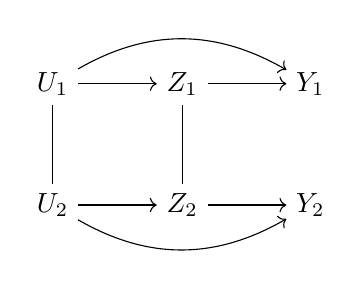
\begin{tikzpicture}
		\node (1) {$U_1$};
		\node[ right= of 1] (2) {$Z_1$};
		\node[ right= of 2] (3) {$Y_1$};
		\node[below = of 1] (12) {$U_2$};
		\node[ right= of 12] (22) {$Z_2$};
		\node[ right= of 22] (32) {$Y_2$};
		\draw[->] (1) to (2);
		\draw[->] (1) to [out=30,in=150] (3);
		\draw[->] (2) to (3); 
		\draw[->] (12) to (22);
		\draw[->] (12) to [out=330,in=210] (32);
		\draw[->] (22) to (32);
		\draw[-] (1) to (12);
		\draw[-] (2) to (22);
	\end{tikzpicture}
\caption{{\bf Direct Spatial Confounding.}
The covariate is a predictor of the exposure and the outcome only locally. Adjusting for the local confounder is necessary for identifying local and interference effects when the exposure is inherently spatial.}
\label{fig:direct}
\end{subfigure}
%
\hspace{20pt}
% INTERFERENCE
\begin{subfigure}[t]{.45\linewidth}
\centering
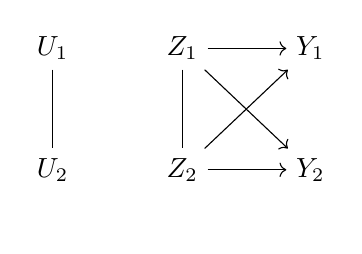
\begin{tikzpicture}
		\node (1) {$U_1$};
		\node[ right= of 1] (2) {$Z_1$};
		\node[ right= of 2] (3) {$Y_1$};
		\node[below = of 1] (12) {$U_2$};
		\node[ right= of 12] (22) {$Z_2$};
		\node[ right= of 22] (32) {$Y_2$};
		\draw[->] (2) to (3); 
		\draw[->] (2) to (32);
		\draw[->] (22) to (3);
		\phantom{\draw[->] (12) to [out=330,in=210] (32);}
		\draw[->] (22) to (32);
		\draw[-] (1) to (12);
		\draw[-] (2) to (22);
	\end{tikzpicture}
\caption{{\bf Spatial interference.}
Unmeasured spatial variables might exist, but they are not confounders. Interference is present as one unit's treatment can affect another unit's outcomes.}
\label{fig:interference}
\end{subfigure}
%
$\ $ \\[30pt]
%
% DIRECT AND INDIRECT SPATIAL CONFOUNDING
\begin{subfigure}[t]{.45\linewidth}
\centering
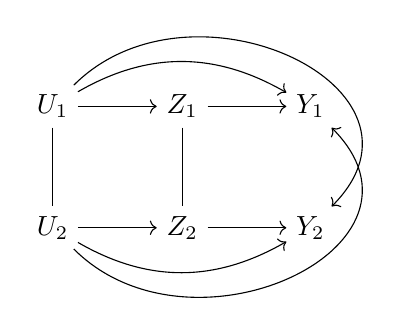
\begin{tikzpicture}
		\node (1) {$U_1$};
		\node[ right= of 1] (2) {$Z_1$};
		\node[ right= of 2] (3) {$Y_1$};
		\node[below = of 1] (12) {$U_2$};
		\node[ right= of 12] (22) {$Z_2$};
		\node[ right= of 22] (32) {$Y_2$};
		\draw[->] (1) to (2);
		\draw[->] (1) to [out=30,in=150] (3);
		\draw[->] (2) to (3); 
		\draw[->] (12) to (22);
		\draw[->] (12) to [out=330,in=210] (32);
		\draw[->] (22) to (32);
		\draw[-] (1) to (12);
		\draw[-] (2) to (22);
	    \clip (0,-2.5) rectangle (4,1);
		\draw[->] (1) to [out=45,in=45,looseness=1.5] (32);
		\draw[->] (12) to [out=315,in=315,looseness=1.5] (3);
	\end{tikzpicture}
\caption{{\bf Direct and Indirect Spatial Confounding.}
The direct spatial confounder is also a predictor of the neighbor's outcome. Local and neighbor's covariate has to be adjusted for identifying local and interference effects.
}
\label{fig:general_spatial_conf}
\end{subfigure}
%
\hspace{20pt}
%
% DIRECT SPATIAL CONFOUNDING AND INTERFERENCE
\begin{subfigure}[t]{.45\linewidth}
\centering
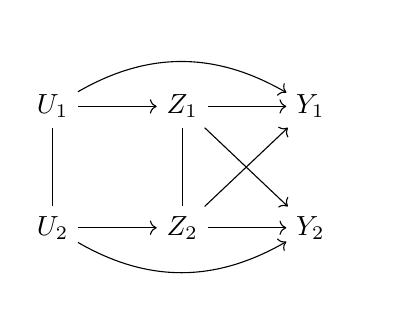
\begin{tikzpicture}
		\node (1) {$U_1$};
		\node[ right= of 1] (2) {$Z_1$};
		\node[ right= of 2] (3) {$Y_1$};
		\node[below = of 1] (12) {$U_2$};
		\node[ right= of 12] (22) {$Z_2$};
		\node[ right= of 22] (32) {$Y_2$};
		\draw[->] (1) to (2);
		\draw[->] (2) to (32);
		\draw[->] (22) to (3);
		\draw[->] (1) to [out=30,in=150] (3);
		\draw[->] (2) to (3); 
		\draw[->] (12) to (22);
		\draw[->] (12) to [out=330,in=210] (32);
		\draw[->] (22) to (32);
		\draw[-] (1) to (12);
		\draw[-] (2) to (22);
		\phantom{
		\clip (0,-2.5) rectangle (4,1);
		\draw[->] (1) to [out=45,in=45,looseness=1.5] (32);
		\draw[->] (12) to [out=315,in=315,looseness=1.5] (3);
		}
	\end{tikzpicture}
\caption{{\bf Direct Spatial Confounding and Interference.} 
Conditioning on both exposure values and the local confounder is necessary for identifying local and interference effects due to the inherent spatial structure in $\bm U$ and $\bm Z$. 
}
\label{fig:direct_interference}
\end{subfigure}
%
$\ $ \\[30pt]
%
% INTERFERENCE ONLY
\begin{subfigure}[t]{.45\linewidth}
\centering
\begin{tikzpicture}
		\node (1) {$U_1$};
		\node[ right= of 1] (2) {$Z_1$};
		\node[ right= of 2] (3) {$Y_1$};
		\node[below = of 1] (12) {$U_2$};
		\node[ right= of 12] (22) {$Z_2$};
		\node[ right= of 22] (32) {$Y_2$};
		\draw[->] (1) to (2);
		\draw[->] (2) to (32);
		\draw[->] (22) to (3);
		\draw[->] (2) to (3); 
		\draw[->] (12) to (22);
		\draw[->] (22) to (32);
		\draw[-] (1) to (12);
		\draw[-] (2) to (22);
		\phantom{
		\clip (0,-2.5) rectangle (4,1);
		\draw[->] (1) to [out=45,in=45,looseness=1.5] (32);
		\draw[->] (12) to [out=315,in=315,looseness=1.5] (3);
		}
	\end{tikzpicture}
\caption{{\bf Interference and a spatial predictor of the exposure.} %Unmeasured spatial variables drive the exposure value but are not confounders since they do not directly predict the outcome. 
If interference is not accounted for, methods that adjust and do not adjust for unmeasured spatial variables will return different estimates, both of which are wrong. Therefore, unaccounted interference would manifest as spatial confounding.
}
\label{fig:predictor_interference}
\end{subfigure}
%
%
\hspace{20pt}
% ALL SPATIAL CONFOUNDING AND INTERFERENCE
\begin{subfigure}[t]{.45\linewidth}
\centering
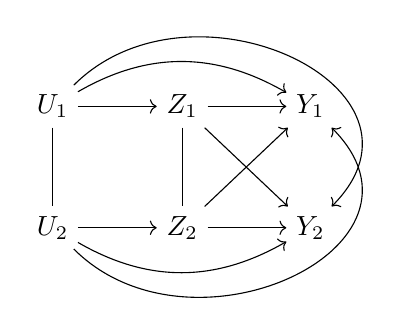
\begin{tikzpicture}
		\node (1) {$U_1$};
		\node[ right= of 1] (2) {$Z_1$};
		\node[ right= of 2] (3) {$Y_1$};
		\node[below = of 1] (12) {$U_2$};
		\node[ right= of 12] (22) {$Z_2$};
		\node[ right= of 22] (32) {$Y_2$};
		\draw[->] (1) to (2);
		\draw[->] (1) to [out=30,in=150] (3);
		\draw[->] (2) to (3); 
		\draw[->] (12) to (22);
		\draw[->] (12) to [out=330,in=210] (32);
		\draw[->] (22) to (32);
		\draw[->] (2) to (32);
		\draw[->] (22) to (3);
		\draw[-] (1) to (12);
		\draw[-] (2) to (22);
	    \clip (0,-2.5) rectangle (4,1);
		\draw[->] (1) to [out=45,in=45,looseness=1.5] (32);
		\draw[->] (12) to [out=315,in=315,looseness=1.5] (3);
	\end{tikzpicture}
\caption{{\bf Direct and Indirect Spatial Confounding with Interference.} The complete graph we consider. Local and interference effects should be investigated simultaneously while also conditioning on the local and neighborhood covariates.
}
\label{fig:general_interference}
\end{subfigure}
\vspace{10pt}
\caption{Graphical representation of spatial confounding and interference in the presence of two units with a spatially correlated variable $\bm U = (U_1, U_2)$, a spatial exposure $\bm Z = (Z_1, Z_2)$, and outcome $\bm Y = (Y_1, Y_2)$.}
\label{fig:graphs}
\end{figure}



% \paragraph{Direct spatial confounding without interference}

The graph in \cref{fig:direct} corresponds to a scenario with {\bf direct spatial confounding and no interference}.
We refer to this confounding structure as direct because it is only the {\it local} value of $U$ that drives the local value for $Y$.
In this setting, there is no interference and $\iota_i(z) = 0$ for all $i$ and $z$. To identify the local causal effects it suffices to control for the local value of the confounder.
%for Unit 1, $\lambda_1(z)$, there are two back-door paths. The first one is the classic back-door path in confounding through the unit's own confounder values, $Z_1 \leftarrow U_1 \rightarrow Y_1$. The second back-door path, $Z_1 - Z_2 \leftarrow U_2 - U_1 \rightarrow Y_1$, is present explicitly due to the inherent spatial dependence in both $\bm Z$ and $\bm U$. Controlling for the local value of the confounder would block both paths and suffice to identify local causal effects.
For estimating the interference effect $\iota_1(z)$, there are three potential back-door paths,
\begin{enumerate*}[label=(\arabic*)]
\item $Z_2 \leftarrow U_2 - U_1 \rightarrow Y_1$ which only exists when $\bm U$ is spatial,
\item $Z_2 - Z_1 \leftarrow U_1 \rightarrow Y_1$ for which $Z_1$ is a collider, and
\item $Z_2 - Z_1 \rightarrow Y_1$.
\end{enumerate*}
Paths (2) and (3) exist specifically due to the inherent spatial structure in the exposure.
If the confounder and the exposure are {\it not} spatial, one could estimate interference effects without any adjustments.
However, even when the confounder is not spatial and path (1) is missing, it is necessary to adjust for the local exposure $Z_1$ {\it and} the local confounder $U_1$ to identify the interference effect on unit 1, $\iota_1(z)$. That is because conditioning on $Z_1$ blocks path (3) but it opens path (2), which in turn can be blocked by conditioning on $U_1$.
% If $\bm Z$ or $\bm U$ were {\it not} spatial, no adjustment would be necessary to estimate interference effects, $\iota_i(z)$. However, 
Therefore, if the exposure variable is inherently spatial, adjusting for the local spatial confounder is necessary for identifying interference effects, and for avoiding mis-attributing spatial statistical dependencies to interference. Even in this simple scenario, we see that the data's inherent spatial dependence ``breaks'' the analysis that would be valid for independent data, and that failing to account for spatial dependencies and confounding could lead researchers to mis-identify spatial interference.

% \paragraph{Interference without spatial confounding}

The graph in \cref{fig:interference} represents a setting with {\bf interference and no spatial confounding}. 
%where the spatial covariates are not confounders, but interference might be present because a unit's outcome can be driven by the neighbor's treatment.
If the exposure variable $\bm Z$ is not spatially-structured (and the edge $Z_1 - Z_2$ is missing), interpretable local and interference effects would be identifiable without any adjustment. For example, the local effect $\lambda_i(\pi)$, for $\pi = P(Z_j = 1)$ would be identifiable simply by comparing the outcomes of Unit $i$ among blocks with $Z_i = 1$ and blocks with $Z_i = 0$, completely ignoring the potential for interference. Similarly, interference effects could be identified without explicitly controlling for the local effects of the treatment. The case is not as simple when $\bm Z$ is inherently spatial. To investigate the local effect for Unit 1, one would necessarily have to account for $Z_2$, since the correlation of $Z_1, Z_2$ and the interference effect of $Z_2$ on $Y_1$ would lead to spurious associations for $Z_1$ and $Y_1$ locally, irrespective the sample size. Therefore, simple analyses that would be justifiable for independent data are no longer applicable in the presence of spatially structured exposure variables.



%\paragraph{Direct and indirect spatial confounding without interference}

The graph in \cref{fig:general_spatial_conf} is a generalization of the one in \cref{fig:direct} that depicts {\bf direct and indirect spatial confounding without interference}. We refer to the situation where a local spatial predictor of the exposure ($U_j \rightarrow Z_j$) drives the outcome in a different location ($U_j \rightarrow Y_i$) as {\it indirect} spatial confounding.
When the exposure is spatial, estimating local effects while adjusting for the neighbor's exposure would open the path $Z_i - Z_j \leftarrow U_j \rightarrow Y_i$ on which $Z_j$ is a collider, and would lead to bias.
Since this path requires that $\bm Z$ is spatially structured, this notion of confounding pertains solely to the setting with dependent data, and it is not met in settings with independent observations.
In this scenario, we would need to adjust for the local and the neighbor's confounder value in order to identify local and interference effects.
% At the same time, to identify the interference effect $\iota_i(z)$, one would need to adjust on the neighbor's confounder value $U_j$ in order to block the backdoor path $Z_j \leftarrow U_j \rightarrow Y_i$.
% The spatial confounder in location $j$, $U_j$, is not a confounder of the local causal effect at location $i$, $\lambda_i(z)$, in the classic sense since it is not a predictor of the exposure at location $i$ (missing arrow from $U_j$ to $Z_i$). Instead, $U_j$ indirectly confounds the $(Z_i, Y_i)$ relationship due to the $Z_i - Z_j \leftarrow U_j \rightarrow Y_i$ path.
% Indirect confounding can occur even if direct confounding does not exist, if for example the local predictor of the exposure is not a predictor of the local outcome ($U_i \rightarrow Z_i$, $U_i \rightarrow Y_j$, but $U_i \not\rightarrow Y_i$).


%\paragraph{Direct confounding with interference}

\cref{fig:direct_interference} shows a setting with {\bf direct spatial confounding and interference}, which combines the scenarios in Figures \ref{fig:direct} and \ref{fig:interference}. When $\bm Z$ is inherently spatial, it is necessary to condition on the local value of the confounder {\it and} the neighbor's exposure to identify local effects. In \cref{supp_sec:identifiability}, we show that if $\bm Z$ is not inherently spatial, interpretable local effects can be identified conditioning only on the local value of the confounder. Similar conclusions can be drawn about the identifiability of interference effects when $\bm Z$ is inherently spatial or not. We again see that the inherent spatial structure in the exposure can lead to misleading conclusions about local and interference effects if not properly accommodated.

%In the case of a spatial exposure ($Z_1-Z_2$), conditioning on the predictors of the exposure alone does not suffice to identify local effects due to the spurious association between $Z_i$ and $Y_i$ that flows through $Z_j$, and the neighbors' exposure value has to be conditioned on as well. Interference effects can be identified conditional only on the local confounder and exposure values.
%In the absence of spatial correlation in the exposure (no edge between $Z_1$ and $Z_2$), the neighbors' exposure will no longer be confounding one's exposure-outcome relationship, and local causal effects can be identified without adjustment for the neighbors' exposure.


The graph in 
\cref{fig:predictor_interference} is a generalization of the graph in \cref{fig:interference} to allow for {\bf interference and a spatial predictor of the exposure}. In this scenario, $\bm U$ is not a confounder for either the local or the interference effect. However, if interference is not accounted for, there is a back-door path from $Z_i$ to $Y_i$, through the unmeasured variable $\bm U$ and the neighbor's exposure $Z_j$. As a result, two methods that both ignore interference, but one adjusts and one does not adjust for the spatial covariate will return different values for the local effect estimate, both of which will be wrong since the path $Z_i - Z_j \rightarrow Y_i$ remains open regardless. Therefore, in this scenario, spatial interference could be mis-interpreted as unmeasured spatial confounding.

%\paragraph{Direct and indirect confounding with interference}

Lastly, the graph in \cref{fig:general_interference} represents the situation also shown in \cref{fig:dag_expanded_considered} with {\bf direct, indirect spatial confounding, and interference}, of which the other graphs are special cases.
%
% It is demonstrated in the figures below that if we do not adjust for the neighbours' spatial confounders, it will lead to incorrect estimates of the neighbours' exposure effect on one's outcome.


\paragraph{}

When dependencies in measured data across locations are present due to missing conditioning variables, one could try to collect more covariate information to ensure that measured data are as close to conditionally independent as possible. However, in spatial settings, variables are inherently dependent, and they will remain dependent irrespective of how many covariates we condition on in our analyses. Therefore, it is paramount that we better comprehend the complications created by the variables' dependence structures in order to separate statistical dependencies from causal relationships, and accurately attribute causal effects. The scenarios considered in \cref{fig:graphs} illustrate that spatial settings are intrinsically different from settings with independent observations, in that confounding and causal dependencies can manifest as each other unless the spatial structure of the data is comprehensively accounted for.


%\clearpage

\subsection{Motivating Simulation Studies in Paired Data}
\label{subsec:illustrate_bias_pairs}

To illustrate the points made above and show how interference and spatial confounding can manifest as each other and affect estimation of local and interference effects, we perform a small simulation study. We simulate pairs of $\bm U$ from a bivariate Normal distribution with mean 0, and covariance matrix $\Sigma_U = \left( \begin{smallmatrix} 1 & \phi_U \\ \phi_U & 1 \end{smallmatrix} \right)$. We also simulate a bivariate normal error term $\bm \epsilon_Z = (\epsilon_{Z,1}, \epsilon_{Z, 2})$ with marginal variances equal to 1 and correlation parameter $\phi_Z$. The binary exposure is generated from a Bernoulli distribution with a logistic link function and linear predictor $\beta_{UZ} U_i + \epsilon_{Z,i}$. Higher values of $\phi_U, \phi_Z$ correspond to stronger inherent spatial dependence for $\bm U$ and $\bm Z$.
Then the outcome is generated independently across pairs and locations according to a normal distribution with linear predictor $\beta_Z Z_i + \beta_{\bar Z} \overline Z_i + \beta_U U_i + \beta_{\bar U} \overline U_i$ and residual variance 1, where we use $\overline Z_i$ and $\overline U_i$ to represent the value of the exposure and the covariate for the neighbor of location $i$, respectively.
We consider the six different scenarios presented in \cref{fig:graphs} by setting different parameters to zero. 
We simulate 300 data sets of 200 pairs each, and fit OLS using different sets of predictor variables.
The data generating model and hyperparameters for each of these scenarios is listed in Table \ref{tab:pairdata}, along with the bias for the least squares estimators of $\beta_Z$ and $\beta_{\bar{Z}}$ which, under this model, correspond to the local and interference effects, respectively.



\begin{table}[!t]
\centering
\caption{Motivating Simulation Study with Paired Data. For the graphs of \cref{fig:graphs}, we illustrate the induced biases in estimating local and interference causal effects due to spatial dependencies.
In these simulations, the parameters that drive the data generative mechanism are $\phi_U, \phi_Z, \beta_{UZ}, \beta_Z, \beta_{\bar Z}, \beta_U, \beta_{\bar U}.$ The different scenarios of \cref{fig:graphs} correspond to different set of parameters fixed at 0, shown below. Unless otherwise noted, these parameters are fixed at $\phi_U = 0.7$, $\phi_Z = 0.5, \beta_{UZ} = 1, \beta_Z = 1, \beta_{\bar Z} = 0.8, \beta_U = 1, \beta_{\bar U} = 0.5$. We generate 300 data sets of 200 pairs each. We regress the outcome on a different set of variables (columns), and report the bias of the OLS estimator for the local effect estimator, $\beta_Z$, and the interference effect estimator, $\beta_{\bar Z}$, when $\overline Z$ is included in the conditioning set. Values are rounded to the third decimal point, and those in {\bf bold} are discussed in the main text.}
    % \rowcolors{5}{}{gray!10}
    \resizebox{0.9\textwidth}{!}{%
    \begin{tabular}{*{10}{c}}
        \hline
        & & & & &  & \\
        & & \multicolumn{8}{c}{Conditioning set} \\
        \cmidrule{3-10} 
        True & Changes in  &  $(Z) $ & $(Z, U)$  & \multicolumn{2}{c}{  $(Z, \bar{Z})$} & \multicolumn{2}{c}{  $(Z, \bar{Z}, U)$} & \multicolumn{2}{c}{  $(Z, \bar{Z}, U, \bar{U})$}\\
        \cmidrule(lr){3-3} \cmidrule(lr){4-4} \cmidrule(lr){5-6} \cmidrule(lr) {7-8} \cmidrule(lr) {9-10}
        Model & spatial parameter & $\beta_Z$ & $\beta_Z$ & $\beta_Z$ & $\beta_{\bar{Z}}$ & $\beta_Z$ & $\beta_{\bar{Z}}$ & $\beta_Z$ & $\beta_{\bar{Z}}$\\
        & & & & & & \\
        \hline \\[-5pt]
%
\multirow{2}{*}{\ref{fig:direct}} & & \multicolumn{8}{c}{$\beta_{\bar Z} = 0$ and $\beta_{\bar U}=0$} \\[5pt]
        \cmidrule{5-8}
        & & 0.726 & -0.003 & 0.660 & {\bf 0.406} & -0.003 & {\bf -0.002} & -0.002 & 0.000  \\
        \midrule \\[-5pt]
%
\multirow{4}{*}{\ref{fig:interference}} & & 
\multicolumn{8}{c}{$\beta_{UZ} = 0$ and $\beta_U = \beta_{\bar U} = 0$}
        \\[5pt]
        \cmidrule{5-8}
        & $\phi_z = 0.7$ & {\bf 0.152} & 0.087 & 0.001 & -0.002 & -0.001 & -0.003 & 0.000 & -0.002  \\
         & $\phi_z = 0.5$ & {\bf 0.129} & 0.060 & -0.001 & -0.001 & -0.003 & -0.002 & -0.002 & 0.000 \\
        & $\phi_z = 0.3$ & {\bf 0.105} & 0.032 & -0.002 & 0.001 & -0.003 & 0.000 & -0.003 & 0.001 \\
        \midrule \\[-5pt]
%
\multirow{2}{*}{\ref{fig:general_spatial_conf}} & & 
        \multicolumn{8}{c}{$\beta_{\bar Z} = 0$}
        \\[5pt]
        \cmidrule{5-8}
%        & $\phi_z = 0.7$ & 0.909 & -0.007 & 0.816 & 0.601 & -0.036 & 0.297 & -0.006 & 0.004 \\ 
         & %$\phi_z = 0.5$ 
         & 0.983 & 0.002 & 0.863 & 0.737 & -0.013 & {\bf 0.198} & -0.002 & {\bf 0.000}  \\ 
%         & $\phi_z = 0.3 $ & 0.904 & -0.008 & 0.839 & 0.636 & -0.020 & 0.295 & -0.005 & 0.004  \\
         \midrule \\[-5pt]
%
\multirow{3}{*}{\ref{fig:direct_interference}} & & 
\multicolumn{8}{c}{$\beta_{\bar U} = 0$} \\[5pt]
        \cmidrule{5-8}
& $\phi_Z = 0.5$ & 0.856 & {\bf 0.060} & 0.660 & 0.406 & -0.003 & -0.002 & -0.002 & 0.000 \\ 
& $\phi_Z = 0\phantom{.5}$ & 0.800 & {\bf -0.001} & 0.684 & 0.445 & 0.000 & -0.003 & 0.000 & -0.001 \\
\midrule \\[-5pt]
%
\multirow{4}{*}{\ref{fig:predictor_interference}} & 
& \multicolumn{8}{c}{$\beta_U = 0$ and $\beta_{\bar U} = 0$} \\[5pt]
\cmidrule{5-8}
        & $\beta_{UZ} = 1.5$ & {\bf 0.173} & {\bf 0.052} & 0.000 & 0.001 & -0.002 & 0.000 & -0.002 & 0.003 \\
        & $\beta_{UZ} = 1\phantom{.a}$ &  0.129 & 0.060 & -0.001 & -0.001 & -0.003 & -0.002 & -0.002 & 0.000  \\
        & $\beta_{UZ} = 0.5$ & 0.083 & 0.061 & -0.004 & -0.003 & -0.006 & -0.004 & -0.005 & -0.003 \\
\midrule \\[-5pt]
%
\ref{fig:general_interference}
         & & 1.113 & 0.064 & 0.863 & 0.737 & -0.013 & 0.198 & -0.002 & 0.000 \\
        & & & & & &  \\
          \hline
        \end{tabular}
     }%
\label{tab:pairdata}
\end{table}

In the presence of only direct spatial confounding (Scenario \ref{fig:direct}), we see that failing to adjust for the local spatial confounder returns biased interference effect estimates ($\beta_{\bar Z}$ in the model with $Z, \overline Z$ in \cref{tab:pairdata}). Therefore, in the presence of inherently spatial data, adjusting for spatial confounders is crucial for learning interference effects, even if spatial confounding is direct only. When spatial confounding is both direct and indirect (Scenario \ref{fig:general_spatial_conf}), adjusting only for the local spatial confounder and exposure values can still return misleading interference effects ($\beta_{\bar Z}$ in the model with $Z, \overline Z, U$), and it is necessary to also account for the neighbor's covariate value. In the presence of interference (Scenario \ref{fig:interference}) and when the exposure is inherently spatial, the local effect estimator is biased when the neighbor's exposure value is not conditioned on, and the bias is larger for stronger spatial dependence. Instead, local and interference effects can be unbiasedly estimated when they are considered simultaneously ($\beta_Z, \beta_{\bar Z}$ in the model with $Z, \overline Z$).
In Scenario \ref{fig:direct_interference}, we see that when the exposure is not inherently spatial ($\phi_Z = 0$), we can learn the local effects without adjusting for the neighbor's exposure. However, this estimator would be biased when the exposure has an inherent spatial structure, illustrating again that spatial dependencies can hinder some analyses invalid if not properly taken into account.
In Scenario \ref{fig:predictor_interference}, the local effect of the exposure for unit $i$ is biased regardless of whether the $U_i$ is adjusted for or not. At the same time, the estimates when $U_i$ is included in the model or not are substantially different, which could be interpreted as $U_i$ confounding the local effect. Therefore, in this scenario, the inherent spatial structure in the confounders and exposure could lead to  interference being mistakenly interpreted as spatial confounding. Of course, when all the possible dependencies are present in Scenario \ref{fig:general_interference}, one would need to condition on everything to properly estimate local and interference effects.

In these motivating simulations we have assumed that the covariate $\bm U$ is measured, and have investigated biases in estimating causal effects when we use different conditioning sets. However, when the confounders required to satisfy \cref{ass:paired_ignorability} are not all measured, biases for estimating local and interference effects persist. In \cref{sec:method}, we discuss a method that aims to mitigate bias due to unmeasured spatial confounders in estimating local and interference effects.




% \paragraph{Simulation results}

% In this section we consider combinations of different true data generating models and fitted models to explore how the treatment effect estimators perform in each situation. Specifically we consider six different simulation scenarios as depicted in Figure 1 and fit linear models which has combinations of the treatment $Z$, the neighbour's treatment $\bar{Z}$, the spatial confounder $U$ and neighbour's spatial confounder $\bar{U}$. 

% In Table \ref{tab:combined} we consider 4 different simulation scenarios and in each scenario we fit different linear models and also the affine estimator. In Table \ref{tab:combined} we want to check that if the true model has only $Z$ and $\bar{Z}$ (and of course $C$) then how does the coefficient of $Z$ changes when we have only $C$ with $Z$ as opposed to having both $U$ and $C$ along with $Z$. For this experiment we have generated $U$ and $Z$ from their joint distribution as done for other rows in the table so as to preserve that dependence of $U$ and $Z$. We expect the coefficient of $Z$ to change when we add $U$ but it will not be better as we not adding the correct term ($\bar{Z}$). This might make us think that there is spatial confounding as we see a change in the coefficient of $Z$ but it is not the spatial confounding but interference in the true model which is the reason behind this change.



% \begin{table}[htbp]
%     \centering
%     \caption{Simulation Results}
%     % \rowcolors{5}{}{gray!10}
%     \resizebox{1.0\textwidth}{!}{%
%     \begin{tabular}{*{5}{c}}
%         \hline
%         True model & Fitted Model (Method) & bias & std error & estimate \\
%         \hline
%         $Y = 1 + 0.8 Z + U + \epsilon$, $\tau_U = 1$  & $Y \sim Z $ (OLS) & 0.6754955878 & 1.2834318 & 1.4754956 \\
%         & $Y \sim Z + \bar{Z} $ (OLS) &  0.5814788284 & 1.2675934 & 1.3814788 \\
%          & $Y \sim Z + U $ (OLS) &  0.0006709997 & 0.9769358 & 0.7993290 \\
%          & $Y \sim Z + \bar{Z} + U $ (OLS) &  -0.0018012268 & 0.9818240 & 0.7981988\\
%          & $Y \sim Z + U$ (affine) & 0.0027154422 & 0.9788643 & 0.8027154 \\
%       \hline
       
%          $Y = 1 + 0.8 Z + 0.4 \bar{Z} + U + \epsilon,$ $\tau_U = 1$  & $Y \sim Z $ (OLS) & 0.784380694 & 1.337471 & 1.5843807\\
%         & $Y \sim Z + \bar{Z} $ (OLS) &  0.581478828 & 1.267593 & 1.3814788 \\
%          & $Y \sim Z + U $ (OLS) &  0.108214107 & 1.002002 & 0.9082141 \\
%          & $Y \sim Z + \bar{Z} + U $ (OLS) &  -0.001801227 & 0.981824 & 0.7981988 \\
%          & $Y \sim Z + U$ (affine) &   0.072002281 & 1.003155 & 0.8720023 \\
        
%         \hline
%          $Y = 1 + 0.8 Z + U + \epsilon,$ $\tau_U = 0.05$  & $Y \sim Z $ (OLS) &  3.0232379077 & 3.7644575 & 3.8232379 \\
%          & $Y \sim Z + \bar{Z} $ (OLS) &  2.6067064798 & 3.6451792 & 3.4067065 \\
%          & $Y \sim Z + U $ (OLS) &  0.0006709997 & 0.9769358 & 0.7993290 \\
%          & $Y \sim Z + \bar{Z} + U $ (OLS) & -0.0018012268 & 0.9818240 & 0.7981988 \\
%          & $Y \sim Z + U$ (affine) &   0.0100933355 & 1.0123496 & 0.8100933 \\
         
%          \hline
         
%         $Y = 1 + 0.8 Z + U + \epsilon,$ $\tau_U = 10$  & $Y \sim Z $ (OLS) & 0.2131516497 & 1.0161609 & 1.0131516 \\
%         & $Y \sim Z + \bar{Z} $ (OLS) &  0.1826481220 & 1.0176842 & 0.9826481\\
%          & $Y \sim Z + U $ (OLS) &  0.0006709997 & 0.9769358 &  0.7993290 \\
%          & $Y \sim Z + \bar{Z} + U $ (OLS) & -0.0018012268 &  0.9818240 & 0.7981988\\
%          & $Y \sim Z + U$ (affine) &   0.0005958585 & 0.9771288 & 0.8005959 \\
     
%         \hline
%     \end{tabular}
%      }%
%      \label{exp1}
% \end{table}

% \begin{table}[htbp]
%     \centering
%     \caption{Simulation Results}
%     % \rowcolors{5}{}{gray!10}
%     \resizebox{0.75\textwidth}{!}{%
%     \begin{tabular}{*{7}{c}}
%         \hline
%         True model & Fitted Model (Method) & bias & std error & estimate of $\beta_z$ & estimate of $\beta_{\bar{z}}$\\
%         \hline
%         & & & & & \\
%          $Y = 1 + 0.8 Z + C + U + \epsilon$   & $Y \sim Z + U + C$ (affine) & -0.0057 & 1.0040 & 0.7943  \\
%           $\rho = 0.5$ & $Y \sim Z + \bar{Z} + U + C$ (affine) & -0.0214 &       1.0155 &  0.7786 & 0.0437  \\
%           & $Y \sim Z +  C$ (OLS) & 0.6604 & 1.2766 & 1.4604 \\
%           & $Y \sim Z + \bar{Z}  + C$ (OLS) & 0.5801 &  1.2651  &  1.3801  &    0.3275 \\
%           & & & & & \\
%          & & & & & \\
%          $Y = 1 + 0.8 Z + C + U + \epsilon$   & $Y \sim Z + U + C$ (affine) & -0.0037 & 0.9940 & 0.7963  \\
%           $\rho = 0.3$ & $Y \sim Z + \bar{Z} + U +C$ (affine) & -0.0216 & 1.0043 & 0.7784 & 0.0426  \\
%           & $Y \sim Z +  C$ (OLS) & 0.3647 & 1.2623 & 1.1648\\
%           & $Y \sim Z + \bar{Z}  + C$ (OLS) & 0.347 & 1.2643  &   1.147  &     0.1842\\
%           & & & & & \\
%          & & & & & \\
%          $Y = 1 + 0.8 Z + C + U + \epsilon$   & $Y \sim Z + U + C$ (affine) & 0.0008 & 0.9907 & 0.7992  \\
%           $\rho = 0.1$ & $Y \sim Z + \bar{Z} + U + C$ (affine) & -0.0222 &       1.0018 & 0.7778 & 0.0389  \\
%           & $Y \sim Z +  C$ (OLS) & 0.1175 & 1.2581 & 0.9175\\
%           & $Y \sim Z + \bar{Z}  + C$ (OLS) &  0.094 & 1.2694  & 0.894  &      0.1002 \\
%           & & & & & \\
%          \hline
%          & & & & & \\
%          $Y = 1 + 0.8 Z + 0.4 \bar{Z} + C + U + \epsilon$ & $Y \sim Z + U + C$ (affine) & 0.0608 & 1.0335 & 0.8608 \\
%          $\rho = 0.5$ & $Y \sim Z + \bar{Z} + U + C$ (affine) & -0.0214  &       1.0155 & 0.7786 & 0.4437 \\
%          & $Y \sim Z +  C$ (OLS) & 0.7638 & 1.3381 & 1.5638\\
%           & $Y \sim Z + \bar{Z}  + C$ (OLS) &  0.561 & 1.2707  & 1.361  &     0.7652\\
%          & & & & & \\
%          & & & & & \\
%          $Y = 1 + 0.8 Z + 0.4 \bar{Z} + C + U + \epsilon$   & $Y \sim Z + U + C$ (affine) & 0.0094 & 1.0143 & 0.8094  \\
%           $\rho = 0.3$ & $Y \sim Z + \bar{Z} + U + C$ (affine) & -0.0216  &       1.0043 &  0.7784  &  0.4426   \\
%           & $Y \sim Z +  C$ (OLS) & 0.4142 & 1.2946 & 1.2142 \\
%           & $Y \sim Z + \bar{Z}  + C$ (OLS) &  0.3258   & 1.2698  &  1.1258 &       0.6272\\
%           & & & & & \\
%           & & & & & \\
%          $Y = 1 + 0.8 Z + 0.4 \bar{Z} + C + U + \epsilon$   & $Y \sim Z + U + C$ (affine) & -0.0026 & 1.0078 & 0.7973\\
%           $\rho = 0.1$ & $Y \sim Z + \bar{Z} + U + C$ (affine) &  -0.0222 &         1.0018 &  0.7778 & 0.4389\\
%           & $Y \sim Z +  C$ (OLS) & 0.1515 & 1.2764 & 0.9515 \\
%           & $Y \sim Z + \bar{Z}  + C$ (OLS) & 0.094 & 1.2694 &  0.894 &      0.5002\\
%           & & & & & \\
%          \hline
%           & & & & & \\
%          $Y = 1 + 0.8 Z + C + U + \bar{U} + \epsilon$  & $Y \sim Z + U + C$ (affine) & 0.0274 & 1.1635 & 0.8274 \\
%          $\rho = 0.5$ & $Y \sim Z + \bar{Z} + U + C$ (affine) & 0.1406 &        1.1934 & 0.9406 & 0.7032 \\
%          & $Y \sim Z +  C$ (OLS) & 0.1564 & 1.4783 & 0.9564\\
%           & $Y \sim Z + \bar{Z}  + C$ (OLS) & 0.723 & 1.5029 & 1.523 & 1.0399 \\
%           & $Y \sim Z + U + \bar{U} + C$ (affine) & -0.0013 & 1.2695 & 0.7987 \\
%           & $Y \sim Z + \bar{Z} + U + \bar{U} +C$ (affine) &  -0.0138  &  1.2791  &  0.7862 &  0.0631  \\
%          & & & & & \\
%           & & & & & \\  
%         $Y = 1 + 0.8 Z + C +  U + \bar{U} + \epsilon$   & $Y \sim Z + U + C$ (affine) &  0.1047 & 1.1817 & 0.9048 \\
%         $\rho = 0.3$ & $Y \sim Z + \bar{Z} + U + C$ (affine) & 0.0733 &       1.1796 & 0.8733 &  0.4267 \\
%         & $Y \sim Z +  C$ (OLS) & 0.5039 & 1.5073 & 1.3038\\
%           & $Y \sim Z + \bar{Z}  + C$ (OLS) &  0.4218  &  1.4953  & 1.2218  &     0.6217\\
%           & $Y \sim Z + U + \bar{U} + C$ (affine) & 0.0021 & 1.1688 & 0.8021 \\
%           & $Y \sim Z + \bar{Z} + U + \bar{U} +C$ (affine) &   -0.0146 & 1.1778 & 0.7854 & 0.0576\\
%         & & & & & \\  
%         & & & & & \\
%          $Y = 1 + 0.8 Z + C + U + \bar{U} + \epsilon$  & $Y \sim Z + U + C$ (affine) & 0.0274 & 1.1635 & 0.8274\\
%          $\rho = 0.1$ & $Y \sim Z + \bar{Z} + U + C$ (affine) &  \\
%          & $Y \sim Z +  C$ (OLS) & 0.1506 & 1.4823 & 0.9506\\
%           & $Y \sim Z + \bar{Z}  + C$ (OLS) & 0.1405 & 1.4805 & 0.9405 & 0.1829 \\
%           & $Y \sim Z + U + \bar{U} + C$ (affine) & 0.0054 & 1.1450 & 0.8054  \\
%           & $Y \sim Z + \bar{Z} + U + \bar{U} +C$ (affine) & -0.0181 & 1.1531 & 0.7819 & 0.0463 \\
%          & & & & & \\
%           \hline  
%         & & & & & \\  
%         $Y = 1 + 0.8 Z + 0.4 \bar{Z} + C +  U + \bar{U} + \epsilon$   & $Y \sim Z + U + C$ (affine) & 0.3606 & 1.3518 & 1.1606 \\
%         $\rho = 0.5$ & $Y \sim Z + \bar{Z} + U + C$ (affine) & 0.1406 &       1.1934 & 0.9406 & 1.1032 \\
%         & $Y \sim Z +  C$ (OLS) & 1.0972 & 1.7193 & 1.8972 \\
%           & $Y \sim Z + \bar{Z}  + C$ (OLS) & 0.723 & 1.5029 & 1.523 & 1.4399 \\
%           & $Y \sim Z + U + \bar{U} + C$ (affine) &  \\
%           & $Y \sim Z + \bar{Z} + U + \bar{U} +C$ (affine) & -0.0138 & 1.2791 &       0.7862 &  0.4631\\
%         & & & & & \\
%         & & & & & \\  
%         $Y = 1 + 0.8 Z + 0.4 \bar{Z} + C +  U +  \bar{U} + \epsilon$   & $Y \sim Z + U + C$ (affine) &  \\
%         $\rho = 0.3$ & $Y \sim Z + \bar{Z} + U + C$ (affine) &  \\
%         & $Y \sim Z +  C$ (OLS) &  \\
%           & $Y \sim Z + \bar{Z}  + C$ (OLS) & \\
%           & $Y \sim Z + U + \bar{U} + C$ (affine) & \\
%           & $Y \sim Z + \bar{Z} + U + \bar{U} +C$ (affine) & \\
%         & & & & & \\
%         & & & & & \\  
%         $Y = 1 + 0.8 Z + 0.4 \bar{Z} + C +  U + \bar{U} + \epsilon$   & $Y \sim Z + U + C$ (affine) & \\
%         $\rho = 0.1$ & $Y \sim Z + \bar{Z} + U + C$ (affine) &  \\
%         & $Y \sim Z +  C$ (OLS) &  \\
%           & $Y \sim Z + \bar{Z}  + C$ (OLS) &  \\
%           & $Y \sim Z + U + \bar{U} + C$ (affine) & \\
%           & $Y \sim Z + \bar{Z} + U + \bar{U} +C$ (affine) & \\
%         & & & & & \\
%          \hline
%         \end{tabular}
%      }%
%      \label{exp2}
% \end{table}

% \begin{table}[htbp]
%     \centering
%     \caption{Simulation Results}
%     % \rowcolors{5}{}{gray!10}
%     \resizebox{0.8\textwidth}{!}{%
%     \begin{tabular}{*{7}{c}}
%         \hline
%         True model & Fitted Model (Method) & bias & std error & estimate of $\beta_z$ & estimate of $\beta_{\bar{z}}$\\
%         \hline
%         & & & & & \\
%          $Y = 1 + 0.8 Z + C + 0.5U + \epsilon$   & $Y \sim Z + U + C$ (affine) &   \\
%           $\rho = 0.5$ & $Y \sim Z + \bar{Z} + U + C$ (affine) &  \\
%           & $Y \sim Z +  C$ (OLS) &  \\
%           & $Y \sim Z + \bar{Z}  + C$ (OLS) &  \\
%           & & & & & \\
%          & & & & & \\
%          $Y = 1 + 0.8 Z + C + 0.5U + \epsilon$   & $Y \sim Z + U + C$ (affine) &  \\
%           $\rho = 0.3$ & $Y \sim Z + \bar{Z} + U +C$ (affine) &  \\
%           & $Y \sim Z +  C$ (OLS) &\\
%           & $Y \sim Z + \bar{Z}  + C$ (OLS) & \\
%           & & & & & \\
%          & & & & & \\
%          $Y = 1 + 0.8 Z + C + 0.5U + \epsilon$   & $Y \sim Z + U + C$ (affine) & \\
%           $\rho = 0.1$ & $Y \sim Z + \bar{Z} + U + C$ (affine) &  \\
%           & $Y \sim Z +  C$ (OLS) & \\
%           & $Y \sim Z + \bar{Z}  + C$ (OLS) &   \\
%           & & & & & \\
%          \hline
%          & & & & & \\
%          $Y = 1 + 0.8 Z + 0.4 \bar{Z} + C + 0.5U + \epsilon$ & $Y \sim Z + U + C$ (affine) &  \\
%          $\rho = 0.5$ & $Y \sim Z + \bar{Z} + U + C$ (affine) & \\
%          & $Y \sim Z +  C$ (OLS) & \\
%           & $Y \sim Z + \bar{Z}  + C$ (OLS) & \\
%          & & & & & \\
%          & & & & & \\
%          $Y = 1 + 0.8 Z + 0.4 \bar{Z} + C + 0.5U + \epsilon$   & $Y \sim Z + U + C$ (affine) &  \\
%           $\rho = 0.3$ & $Y \sim Z + \bar{Z} + U + C$ (affine) &  \\
%           & $Y \sim Z +  C$ (OLS) &  \\
%           & $Y \sim Z + \bar{Z}  + C$ (OLS) &  \\
%           & & & & & \\
%           & & & & & \\
%          $Y = 1 + 0.8 Z + 0.4 \bar{Z} + C + 0.5U + \epsilon$   & $Y \sim Z + U + C$ (affine) & \\
%           $\rho = 0.1$ & $Y \sim Z + \bar{Z} + U + C$ (affine) &  \\
%           & $Y \sim Z +  C$ (OLS) &  \\
%           & $Y \sim Z + \bar{Z}  + C$ (OLS) & \\
%           & & & & & \\
%          \hline
%           & & & & & \\
%          $Y = 1 + 0.8 Z + C + U + 0.5 \bar{U} + \epsilon$  & $Y \sim Z + U + C$ (affine) & 0.1301 & 1.0755 & 0.9301 \\
%          $\rho = 0.5$ & $Y \sim Z + \bar{Z} + U + C$ (affine) & 0.0597 &        1.0708 &  0.8597 & 0.3724 \\
%          & $Y \sim Z +  C$ (OLS) & 0.8271 & 1.4090 & 1.6271\\
%           & $Y \sim Z + \bar{Z}  + C$ (OLS) &  0.642 & 1.3625 & 1.442 &      0.7026\\
%          & & & & & \\
%           & & & & & \\  
%         $Y = 1 + 0.8 Z + C +  U +  0.5 \bar{U} + \epsilon$   & $Y \sim Z + U + C$ (affine) &   \\
%         $\rho = 0.3$ & $Y \sim Z + \bar{Z} + U + C$ (affine) & 0.0258  &       1.0591 & 0.8258 & 0.234 \\
%         & $Y \sim Z +  C$ (OLS) & \\
%           & $Y \sim Z + \bar{Z}  + C$ (OLS) & 0.3738 & 1.3589 & 1.1738 & 0.4245\\
%         & & & & & \\  
%         & & & & & \\
%          $Y = 1 + 0.8 Z + C + U + 0.5 \bar{U} + \epsilon$  & $Y \sim Z + U + C$ (affine) & \\
%          $\rho = 0.1$ & $Y \sim Z + \bar{Z} + U + C$ (affine) & -0.0053 &          1.056 & 0.7947 & 0.1055 \\
%          & $Y \sim Z +  C$ (OLS) & \\
%           & $Y \sim Z + \bar{Z}  + C$ (OLS) & 0.1111 & 1.3575  &  0.9111 &      0.1696 \\
%          & & & & & \\
%           \hline  
%         & & & & & \\  
%         $Y = 1 + 0.8 Z + 0.4 \bar{Z} + C +  U +  0.5 \bar{U} + \epsilon$   & $Y \sim Z + U + C$ (affine) & 0.2144 & 1.1518 & 1.0144 \\
%         $\rho = 0.5$ & $Y \sim Z + \bar{Z} + U + C$ (affine) & 0.0596  &       1.0707  & 0.8596 & 0.7722 \\
%         & $Y \sim Z +  C$ (OLS) & 0.9399 & 1.5043 & 1.7399 \\
%           & $Y \sim Z + \bar{Z}  + C$ (OLS) & 0.642 & 1.3625 & 1.442  &     1.1026 \\
%         & & & & & \\
%         & & & & & \\  
%         $Y = 1 + 0.8 Z + 0.4 \bar{Z} + C +  U +  0.5 \bar{U} + \epsilon$   & $Y \sim Z + U + C$ (affine) & 0.06512 & 1.0897 & 0.8651  \\
%         $\rho = 0.3$ & $Y \sim Z + \bar{Z} + U + C$ (affine) & 0.0258 &       1.059 & 0.8258 & 0.6339 \\
%         & $Y \sim Z +  C$ (OLS) & 0.4837 & 1.4043 & 1.2837 \\
%           & $Y \sim Z + \bar{Z}  + C$ (OLS) & 0.3738 &  1.3589 & 1.1738 &      0.8245\\
%         & & & & & \\
%         & & & & & \\  
%         $Y = 1 + 0.8 Z + 0.4 \bar{Z} + C +  U +  0.5 \bar{U} + \epsilon$   & $Y \sim Z + U + C$ (affine) & 0.0134 & 1.0663 & 0.8134 \\
%         $\rho = 0.1$ & $Y \sim Z + \bar{Z} + U + C$ (affine) & -0.0053 & 1.056 &    0.7947  &  0.5055 \\
%         & $Y \sim Z +  C$ (OLS) & 0.1709 & 1.3661 & 0.9709 \\
%           & $Y \sim Z + \bar{Z}  + C$ (OLS) & 0.1111 & 1.3575  &  0.9111 &      0.5696 \\
%         & & & & & \\
%          \hline
%         \end{tabular}
%      }%
%      \label{exp3}
% \end{table}

% \begin{table}[htbp]
%     \centering
%     \caption{Simulation Results}
%     % \rowcolors{5}{}{gray!10}
%     \resizebox{0.9\textwidth}{!}{%
%     \begin{tabular}{*{5}{c}}
%         \hline
%         True model & Fitted Model (Method) & bias & std error & estimate of $\beta_z$ \\
%         \hline
%         & & & &  \\
%         $Y = 1 + 0.8 Z + 0.4 \bar{Z} + C + \epsilon$   & $Y \sim Z + C$ (OLS) & -0.0021 & 0.9983 & 0.7979   \\
%           $\rho = 0.5$ & $Y \sim Z + U + C$ (affine) & -0.6203 & 0.7463 & 0.1797 \\
%           & & & &   \\
%           & & & &  \\
%          $Y = 1 + 0.8 Z + 0.4 \bar{Z} + C + \epsilon$   & $Y \sim Z + C$ (OLS) & 0.0005 & 0.9985 & 0.7995  \\
%           $\rho = 0.3$ & $Y \sim Z + U + C$ (affine) & -0.3413 & 0.7142 &  0.4587 \\
%           & & & &   \\
%           & & & &  \\
%          $Y = 1 + 0.8 Z + 0.4 \bar{Z} + C + \epsilon$   & $Y \sim Z + C$ (OLS) & 0.0012 & 0.9986 & 0.8012   \\
%           $\rho = 0.1$ & $Y \sim Z + U + C$ (affine) & -0.1077 &  0.7070 & 0.6923 \\
%           & & & &   \\
%           \hline
%         \end{tabular}
%      }%
%      \label{exp4}
% \end{table}

% \begin{table}[htbp]
%     \centering
%     \caption{Simulation Results}
%     % \rowcolors{5}{}{gray!10}
%     \resizebox{0.9\textwidth}{!}{%
%     \begin{tabular}{*{5}{c}}
%         \hline
%         True model & Fitted Model (Method) & bias & std error & estimate of $\beta_z$ \\
%         \hline
%         & & & &  \\
%         $Y = 1 + 0.8 Z + 0.4 \bar{Z} + C + \epsilon$   & $Y \sim Z + C$ (OLS) &   0.0352 & 1.0164 & 0.8352\\
%           $\rho = 0.5$ & $Y \sim Z + \bar{Z} + C$ (OLS) & 0.0034 & 0.9985 & 0.8034\\
%           & $Y \sim Z + U + C$ (affine) & -0.1264 & 0.7229 & 0.6736  \\
%           & & & &   \\
%           & & & &  \\
%          $Y = 1 + 0.8 Z + 0.4 \bar{Z} + C + \epsilon$   & $Y \sim Z + C$ (OLS) & 0.0345 & 1.0163 & 0.8345  \\
%           $\rho = 0.3$ & $Y \sim Z + \bar{Z} + C$ (OLS) &  0.0033 & 0.9985 & 0.8033\\
%           & $Y \sim Z + U + C$ (affine) & -0.0989 & 0.7211 & 0.7011 \\
%           & & & &   \\
%           & & & &  \\
%          $Y = 1 + 0.8 Z + 0.4 \bar{Z} + C + \epsilon$   & $Y \sim Z + C$ (OLS) & 0.0339 & 1.0163 & 0.8339   \\
%           $\rho = 0.1$ & $Y \sim Z + \bar{Z} + C$ (OLS) & 0.0031 & 0.9985 & 0.8032 \\
%           & $Y \sim Z + U + C$ (affine) & -0.0772 & 0.7205 & 0.7228 \\
%           & & & &   \\
%           \hline
%         \end{tabular}
%      }%
%      \label{exp4}
% \end{table}


% \begin{table}[htbp]
%     \centering
%     \caption{Simulation Results (same as above except $z = z+1$)}
%     % \rowcolors{5}{}{gray!10}
%     \resizebox{0.9\textwidth}{!}{%
%     \begin{tabular}{*{5}{c}}
%         \hline
%         True model & Fitted Model (Method) & bias & std error & estimate of $\beta_z$ \\
%         \hline
%         & & & &  \\
%         $Y = 1 + 0.8 Z + 0.4 \bar{Z} + C + \epsilon$   & $Y \sim Z + C$ (OLS) & 0.10880 & 1.03836 & 0.9088   \\
%           $\rho = 0.5$ & $Y \sim Z + \bar{Z} + C$ (OLS) & -0.0017 & 1.0082 & 0.7983\\
          
%           & & & &   \\
%           & & & &  \\
%          $Y = 1 + 0.8 Z + 0.4 \bar{Z} + C + \epsilon$   & $Y \sim Z + C$ (OLS) &  0.0592 & 1.03097 & 0.8592\\
%           $\rho = 0.3$ & $Y \sim Z + \bar{Z} + C$ (OLS) & 0.000359 & 1.0081 & 0.7996  \\
         
%           & & & &   \\
%           & & & &  \\
%          $Y = 1 + 0.8 Z + 0.4 \bar{Z} + C + \epsilon$   & $Y \sim Z + C$ (OLS) &   0.0440 & 1.02860 & 0.8440\\
%           $\rho = 0.1$ & $Y \sim Z + \bar{Z} + C$ (OLS) & 0.000067 & 1.0080 & 0.80007 \\
          
%           & & & &   \\
%           \hline
%         \end{tabular}
%      }%
%      \label{exp4}
% \end{table}

% \begin{table}[htbp]
%     \centering
%     \caption{Bias of the estimates of the model coefficients where the true model is given by $Y = 1 + 0.8 Z + 0.4 \bar{Z} + C + \epsilon$ and the spatial parameter $\rho$ varies over the set XX. The other spatial parameters ($\phi_U, \phi_Z, \tau_U, \tau_Z$) are fixed at $\phi_{U} = 0.6, \phi_{Z} = 0.6, \tau_U = \tau_Z = 1$}
%     % \rowcolors{5}{}{gray!10}
%     \resizebox{0.9\textwidth}{!}{%
%     \begin{tabular}{*{6}{c}}
%         \hline
%         & & & & & \\
%         Changes in spatial parameter &  $Y \sim Z + C$ & \multicolumn{2}{c}{ $Y \sim Z + U + C$}  & \multicolumn{2}{c}{  $Y \sim Z + \bar{Z} + C$} \\
%         & $Z$ & $Z$ & $U$ & $Z$ & $\bar{Z}$ \\
%         \hline
%         & & & & & \\
%         $\rho = 0.5$ & & & & & \\
%         $\rho = 0.3$ & 0.192 & 0.154 & 0.071 & -0.001 & 0.002 \\
%         $\rho = 0.2$ & 0.151 & 0.136 & 0.044 & -0.001 & 0.002 \\
%         $ \rho = 0.1$ & 0.132 & 0.127 & 0.024 & -0.001 & 0.002 \\
%           \hline
%         \end{tabular}
%      }%
%      \label{tab:bias:1e}
% \end{table}

% \begin{table}[htbp]
%     \centering
%     \caption{Bias of the estimates of the model coefficients where the true model is given by $Y = 1 + 0.8 Z + U + 0.5 \bar{U} + C + \epsilon$ and the spatial parameter $\phi_Z$ varies over the set XX. The other spatial parameters ($\phi_U, \rho, \tau_U, \tau_Z$) are fixed at $\phi_{U} = 0.6, \rho = 0.2 , \tau_U = \tau_Z = 1$}
%     % \rowcolors{5}{}{gray!10}
%     \resizebox{0.6\textwidth}{!}{%
%     \begin{tabular}{*{2}{c}}
%         \hline
%         &  \\
%         Changes in spatial parameter &  Bias of $\hat{\beta}_Z$\\
%         \hline
%         & \\
%         $\phi_Z = 0.9$ & -0.001\\
%         $\phi_Z = 0.6$ & -0.002 \\
%         $\phi_Z = 0.3$ & -0.001  \\
%         $\phi_Z = 0.2$ & -0.001 \\
%         $\phi_Z = 0.1$ & -0.001\\
%           \hline
%         \end{tabular}
%      }%
%      \label{exp4}
% \end{table}

% \begin{table}[htbp]
%     \centering
%     \caption{Simulation Results}
%     % \rowcolors{5}{}{gray!10}
%     \resizebox{1.0\textwidth}{!}{%
%     \begin{tabular}{*{7}{c}}
%         \hline
%         True model & Fitted Model (Method) & bias & std error & estimate of $\beta_z$ & estimate of $\beta_{\bar{z}}$\\
%         \hline
%         & & & & & \\
%         $Y = 1 + 0.8 Z + U + \bar{U} + C + \epsilon$   & $Y \sim Z + U + \bar{U} + C$ (affine) & -0.0013 & 1.2695 & 0.7987 \\
%           $\rho = 0.5$ & $Y \sim Z + \bar{Z} + U + \bar{U} +C$ (affine) &  -0.0138  &  1.2791  &  0.7862 &  0.0631  \\
%           & & & & &  \\
%           & & & & & \\
%          $Y = 1 + 0.8 Z + U + \bar{U} + C + \epsilon$   & $Y \sim Z + U + \bar{U} + C$ (affine) & 0.0021 & 1.1688 & 0.8021 \\
%           $\rho = 0.3$ & $Y \sim Z + \bar{Z} + U + \bar{U} +C$ (affine) &   -0.0146 & 1.1778 & 0.7854 & 0.0576\\
%           & & & & &  \\
%           & & & & & \\
%          $Y = 1 + 0.8 Z + U + \bar{U} + C + \epsilon$   & $Y \sim Z + U + \bar{U} + C$ (affine) & 0.0054 & 1.1450 & 0.8054  \\
%           $\rho = 0.1$ & $Y \sim Z + \bar{Z} + U + \bar{U} +C$ (affine) & -0.0181 & 1.1531 & 0.7819 & 0.0463 \\
%           & & & & &  \\
%           \hline
%         \end{tabular}
%      }%
%      \label{exp4}
% \end{table}




\subsection{Blocked interference with more than two units}
\label{subsec:blocks_larger}

For interference blocks that are larger than two units, estimands for local and interference effects can be defined to average over hypothetical distributions of the neighbors' treatments, in agreement to literature on partial interference \citep{Hudgens2008, Tchetgen2012}.
We define the average outcome for unit $i$ when its treatment is set to a fixed value $z \in \{0, 1\}$, and the treatment of the other units in the block, $\bm z_{-i}$, are independent draws from a Bernoulli distribution with probability of success $\pi \in [0, 1]$ as
\(
\overline Y_i(z, \pi) % & \equiv Y_i(z_i = z, \bm z_{-i} \sim \text{Bern}(\pi)) \\
= \sum_{\bm z_{-i} } Y_i(z_i = z, \bm z_{-i}) p(\bm z_{-i} ; \pi),
\)
where $p(\cdot ; \pi)$ is the joint probability mass function for independent Bernoulli trials with probability of success $\pi$. Then, the local effect for unit $i$ can be defined as
\(
\lambda_i(\pi) = \E \left[ \overline Y_i(1, \pi) - \overline Y_i(0, \pi) \right],
%\label{eq:local_effect_pi}
\)
and the interference effect on unit $i$ as
\(
\iota_i(\pi, \pi'; z) = \E \left[ \overline Y_i(z, \pi') - \overline Y_i(z, \pi) \right].
%\label{eq:interference_effect_pi}
\)
For $\pi, \pi' \in \{0, 1\}$ and for blocks with two units, these estimands revert back to the estimands in \cref{eq:local_effect} and \cref{eq:interference_effect}, respectively.

Spatial dependence in confounders and exposure values will lead to the same complications in identifying local and interference effects discussed for paired data. To avoid distraction, we do not delve into blocked data with more than two units further. Instead, in \cref{sec:one_network} we focus on data on a single spatial network.



\section{Causal inference with spatial dependencies on a single network}
\label{sec:one_network}

In the case of a single network of interconnected units, the population of interest cannot be partitioned in non-interacting groups \citep{aronow2017estimating, Tchetgen2017auto, forastiere2021identification, ogburn2022causal}.
Here, defining and estimating causal effects is more challenging. Again, we will refer to a ``local effect'' if it corresponds to an effect of treating one location on the outcome at the same location, and to an ``interference effect'' if it corresponds to the effect on a location's outcome for a change in the neighbors' treatment.

\subsection{Potential outcomes based on network connections and exposure mapping}
\label{subsec:po_network}

For units $i = 1, 2, \dots, n$, let $Z_i$ denote the treatment value of unit $i$, where $Z_i \in \mathcal{Z}$ can be binary or continuous. Continuous treatments are often referred to as ``exposures,'' so we use the two terms interchangeably.  In full generality, a unit's potential outcomes depend on the treatment level of all other units on the network. Therefore, we assume that there exist potential outcomes $Y_i(\bm z)$ for $\bm z \in \mathcal{Z}^n$ a vector of length $n$ with exposure values on the $n$ units. 
%By decomposing the treatment vector $\bm z$ in unit $i$'s treatment and the treatment of all others $\bm z = (z_i, \bm z_{-i})$, potential outcomes can also be denoted as $Y_i(z_i, \bm z_{-i})$.
We reduce the number of possible potential outcomes by assuming the presence of a known interference network and exposure mapping \citep{aronow2017estimating, zigler2020bipartite, forastiere2021identification}. Let $A$ denote a known adjacency matrix of dimension $n \times n$, where $A_{ij} = 1$ reflects that units $i$ and $j$ are connected, and $A_{ij} = 0$ otherwise. 
%We set the diagonal elements, $A_{ii}$, to 0
%We use $A_{i(-i)}$ to denote the $i^{th}$ row of the matrix excluding the diagonal element, therefore reflecting unit $i$'s connections.
We assume that unit $i$'s potential outcomes depend on its own treatment value, and a function of the treatments for units with which $i$ is connected through $A$. For binary treatments, commonly used functions include the number and proportion of treated neighbors. For simplicity, in what follows we assume that this function corresponds to the average exposure value among the neighbors, which can be applicable for both binary and continuous exposures.

\begin{assumption}
% Let $g:\mathcal{Z}^{n - 1} \times \{0, 1\}^{n - 1} \rightarrow \mathcal{E}$ denote a known function that maps the treatment vector and vector of connections for $n - 1$ units to an exposure value in $\mathcal{E}$.
Let $\bm z, \bm z'$ be two treatment vectors in $\mathcal{Z}^n$ such that $z_i = z_i'$ and $\overline z_i = \overline z_i'$, where $\overline z_i = \sum_{j \neq i} A_{ij} z_j / \sum_{j \neq i}A_{ij},$ and similarly for $\overline z_i'$. Then, it holds that $Y_i(\bm z) = Y_i(\bm z')$, and potential outcomes can be denoted as $Y_i(z_i, \overline z_i).$
\label{ass:sutva}
\end{assumption}

For areal data, considering $A$ being a binary adjacency matrix often makes sense. For the case of point-referenced data however, the adjacency matrix could be alternatively defined such that element $(i, j)$ of the matrix $A$ is equal to $f(d_{ij})$ where $d_{ij}$ is the geographical distance of locations $i$ and $j$, and $f$ is a pre-specified decreasing function (with zeros on the diagonal). Then, the average neighborhood exposure in \cref{ass:sutva} would be a weighted average of the exposures of other locations, with weights driven by the locations' geographic proximity.


\subsection{Ignorability in terms of unmeasured and measured covariates}

For the $n$ units in the network, we assume that there exist $p$ measured covariates $\widetilde C_i = (C_{i1}, C_{i2}, \dots, C_{ip_c})^T$, $i = 1, 2, \dots, n$, which can include unit $i$'s individual covariates, or covariates corresponding to unit $i$'s neighborhood. However, these covariates are not a sufficient conditioning set for unconfoundedness of the treatment assignment.
Specifically, 
\[
(Z_i, \overline Z_i) \not\!\indep Y_i(z, \overline z) \mid \widetilde C_i.
\]
We assume however that unconfoundedness holds conditional on measured covariates, and the local and neighborhood value of an unmeasured covariate.
\begin{assumption}[Ignorability conditional on unmeasured local and neighborhood covariate]
There exists unmeasured covariate $\bm U = (U_1, U_2, \dots, U_n)$ such that
\[
(Z_i, \overline Z_i) \indep Y_i(\cdot) \mid \widetilde C_i, U_i, \overline U_i,
\]
where $Y_i(\cdot) = \{ Y_i(z, \overline z) \text{ for all } z, \overline z\}$ is the collection of unit $i$'s potential outcomes, and $\overline U_i$ is the average value of $U$ in the neighborhood of $i$, $U_i = \sum_{j \neq i} A_{ij}U_j / \sum_{j \neq i} A_{ij}$.
Also, it holds that $f(Z_i = z, \overline Z_i = \overline z_i \mid \widetilde C_i, U_i, \overline U_i) > 0$.
\label{ass:network_ignorability}
\end{assumption}

\paragraph{}
The \cref{ass:sutva} on the potential outcomes and the ignorability \cref{ass:network_ignorability} are in-line with the definition of potential outcomes and the ignorability assumption for paired data discussed in \cref{sec:pairs}. In the case of paired data, the matrix $A$ is in the form of a blocked diagonal matrix with blocks of size two, the average neighborhood exposure $\overline z_i$ corresponds to the neighbor's treatment $z_j$, and the average neighborhood confounder $\overline u_i$ corresponds to the neighbor's covariate value $u_j$. Therefore, the potential outcomes $Y_i(z_i, \overline z_i)$ reduce to $Y_i(z_i, z_j)$, and the independence assumption in \cref{ass:network_ignorability} reduces to the independence statement in \cref{ass:paired_ignorability}, with the addition of measured covariates. Therefore, the estimands described in \cref{subsec:sem_estimands} and estimation procedure in \cref{sec:method} apply both to network and paired data, with the appropriate definition of the adjacency matrix $A$.



\subsection{Local and interference effects within a structural equation modeling framework}
\label{subsec:sem_estimands}

We discuss estimands of interest within the realm of a structural equation model for the potential outcomes. 
Specifically, we assume that the potential outcomes arise according to
\begin{equation}
Y_i(z, \overline z) = f_1(z, \overline z) + f_2(\widetilde C_i) + f_3(U_i, \overline U_i) + \epsilon(z, \overline z)
\label{eq:sem}
\end{equation}
where $f_1, f_2, f_3$ are known functions, and $\epsilon(z, \overline z)$ are mean zero random variables, independent of all others. We assume that all of $f_1, f_2, f_3$ are linear, though non-linear functions could be easily accommodated. Therefore, we assume that the potential outcomes follow a linear structural equation model, written as
\begin{equation}
Y_i(z, \overline z) = \beta_0 + \beta_Z z + \beta_{\bar Z} \overline z + \widetilde C_i^T \bm \beta_C + \beta_U U_i + \beta_{\bar U} \overline U_i + \epsilon(z, \overline z).
\label{eq:linear_sem}
\end{equation}
According to this model, $\beta_Z$ and $\beta_{\bar Z}$ describe the local and interference effects of the exposure, respectively, where the local effect describes the expected change in a unit's outcome for a unit increase in its own exposure when the neighborhood exposure remains fixed, and the interference effect describes the expected change in a unit's outcome for a unit increase in its neighborhood exposure when its individual exposure remains fixed. In the absence of interactions between $z, \overline z$, the local and interference effects do not vary with the level at which we fix the neighborhood and individual exposure, respectively, and in the absence of interactions between the exposure variables and the covariates, the causal effects are constant as a function of an individual's characteristics.
The definitions of local and interference effects according to \cref{eq:linear_sem} agree with the corresponding definitions given in \cref{sec:pairs} for paired data with a binary treatment, and $\beta_Z = \lambda_i(z)$ and $\beta_{\bar Z} = \iota_i(z)$ for both $i$ and $z$.

Structural equation models have been previously employed for defining causal estimands in spatial settings with unmeasured confounders \citep{schnell2020mitigating, christiansen2022toward, papadogeorgou2022discussion}, interference \citep{giffin2022generalized}, or both \citep{giffin2021instrumental}, though model-free definitions using potential outcomes directly have also been employed \citep[e.g.][]{Verbitsky-savitz2012, Gilbert2021approaches}.

% \cite{sobel2014causal, vanderlaan2014causal}


\subsection{Bias in estimating causal effects in the presence of unmeasured spatial confounding, spatial dependence, and interference}
\label{subsec:illustrate_bias_network}

Whether the coefficients in \cref{eq:linear_sem} are zero or not can be conceived in the same manner as to whether some of the arrows are missing or not in the graphs of \cref{fig:graphs}. For example, the structural model for $\beta_{\bar Z} = \beta_{\bar U} = 0$ is consistent with a graph equivalent to that in \cref{fig:direct} with all $n$ units depicted. Under the different scenarios of \cref{fig:graphs}, the ignorability \cref{ass:network_ignorability} might also hold conditional on $\widetilde C$ only, conditional on $\widetilde C$ and $U$, or might only hold as stated conditional on all of $\widetilde C, U$ and $\overline U$, as illustrated in the motivating simulation study of \cref{subsec:illustrate_bias_pairs}.

In the network setting, we provide an example of how the inherent spatial structure that the variables exhibit might occur, without requiring this structure in what follows. We return to viewing the inherent spatial structure in $\bm U$ and $\bm Z$ as driven from underlying covariates $U^u, Z^u$ as in \cref{fig:dag_underlying}. Let $U^u$ be a vector of length $n$, $U^u = (U_1^u, U_2^u, \dots, U_n^u)$ of independent random variables and set $U_i = \sum_{j = 1}^n w_{ij} U_j^u + \epsilon_{i}$, for $w_{ij}$ not all zeros and $\epsilon_i$ independent errors. Then the elements of $\bm U$ that share elements of $U^u$ would be statistically dependent. If the choice of weights $w_{ij}$ is based on the spatial proximity of $i$ and $j$, this dependence structure will be {\it spatially} driven. We can similarly conceive $Z^u$.

In Supplement \ref{supp_sec:motivating_one_network}, we show results based on a motivating simulation study investigating the influence of spatial dependencies in learning local and interference effects for units on a single interconnected network. The conclusions are the same as the ones in \cref{subsec:illustrate_bias_pairs}: spatial confounding and interference can manifest as each other, inherent spatial dependencies complicate standard estimation strategies, and controlling for local and neighborhood covariates is crucial for adjusting for confounding and estimating causal effects unbiasedly. 

When the necessary covariates for confounding adjustment are not all measured, adjusting for the measured covariates only is not sufficient for estimating causal effects. Even if the unmeasured covariate is spatial, including a spatial random effect in the outcome regression will not necessarily reduce bias from unmeasured confounders \citep{schnell2020mitigating, reich2021review}. When the missing confounder exhibits an inherent spatial structure, our approach in \cref{sec:method} mitigates bias due to local and neighborhood unmeasured spatial confounding for estimating local and interference effects.



\section{Bayesian inference of local and interference effects in the presence of spatial dependencies and unmeasured spatial confounding}
\label{sec:method}

Up until now we have focused on the complications of defining and estimating causal quantities in spatial settings with unmeasured confounding, interference, and inherent spatial structures. In what follows, we turn our attention to an estimation strategy that aims to address these complications. Specifically, we develop a Bayesian approach for estimating causal effects in the presence of spatial dependencies in the exposure variable and unmeasured spatial confounding. In \cref{subsec:bayesian_treatment}, we illustrate that the treatment assignment mechanism has to be incorporated in the Bayesian procedure in the presence of missing confounders.
%By viewing the inherent spatial structure in the confounder and the exposure as underlying, unobservable covariates as in \cref{fig:dag_underlying}, we investigate the impact of spatial structure and unmeasured confounding within the Bayesian framework for causal inference.
Based on these derivations, we assume a known structure for the relationship of the unmeasured confounder and the exposure in \cref{subsec:UZ_assumptions}. 
In \cref{subsec:priors}, we discuss the choice of prior distributions for the hyperparameters of the spatial confounder by linking them to its confounding strength.



\subsection{The role of the treatment assignment mechanism under spatial dependencies and unmeasured spatial confounding}
\label{subsec:bayesian_treatment}


Bayesian causal inference views unobserved potential outcomes as missing data, and inference on causal effects is acquired from their posterior distribution \citep{rubin1978bayesian, imbens1997bayesian, ding2018causal, li2022bayesian}.
Let $\bm Z = (Z_1, Z_2, \dots, Z_n)$ denote the vector of length $n$ of realized exposures, $\overline{\bm Z} = (\overline Z_1, \overline Z_2, \dots, \overline Z_n)$ the vector of neighborhood exposures, $\bm C = (\widetilde C_1, \widetilde C_2, \dots, \widetilde C_n)$ the $n \times p_c$ matrix of measured covariates, and
$\bm Y(\cdot)  = \{Y_i (\cdot), \text{ for all } i \} $ the collection of all potential outcomes for all units and possible individual and neighborhood exposures.
Let $\bm Y(\cdot) = \{ \bm Y, \bm Y^{\text{miss}} \}$ where $\bm Y^{\text{miss}}$ denotes the collection of {\it un}observed potential outcomes, and $\bm Y = (Y_1, Y_2, \dots, Y_n)$ the observed outcomes.
% Here, it is helpful to return to \cref{fig:dag_underlying}, and think of the spatial structure in $\bm U, \bm Z$ as driven by underlying variables $U, Z$ that are unobservable. Therefore, all inherent spatial dependent in $\bm U, \bm Z$ is captured by $U, Z$. Conditional on $U, Z$ we assume unit-exchangeability \citep{de1937foresight}, which allows us to write
% \begin{align*}
% p(\bm Y(\cdot), \bm Z, \overline{\bm Z}, \bm C ) &=
% \int p(\bm Y(\cdot), \bm Z, \overline{\bm Z}, \bm C \mid U, Z) \ p(U, Z) \ \mathrm{d}U \mathrm{d}Z \\
% &= \int \prod_{i = 1}^n p(\bm Y_i(\cdot), Z_i, \overline Z_i, \widetilde C_i \mid U, Z, \theta) \ p(\theta \mid U, Z) \ \mathrm{d}\theta \ p(U, Z) \ \mathrm{d}U \mathrm{d}Z \\
% &= \int \prod_{i = 1}^n p(\bm Y_i(\cdot), Z_i, \overline Z_i, \widetilde C_i \mid U, Z, \theta) \ p(U, Z \mid \theta) \ p(\theta) \  \mathrm{d}U \mathrm{d}Z \mathrm{d}\theta
% \end{align*}
% for some vector of parameters $\theta$.
Bayesian inference proceeds by specifying
\(
p(\bm Y(\cdot), \bm Z, \overline{\bm Z}, \bm C \mid \theta)
\) 
and prior distribution \( p(\theta) \),
and imputing missing potential outcomes from
\begin{align*}
p(\bm Y^{\text{miss}} \mid \bm Y, \bm Z, \overline{\bm Z}, \bm C, \theta)
\propto & \ P(\bm Y(\cdot) , \bm Z, \overline{\bm Z}, \bm C \mid \theta) \\
\propto & \ P(\bm Z, \overline{\bm Z} \mid \bm Y(\cdot), \bm C, \theta) \  P(\bm Y(\cdot) \mid \bm C, \theta) \ P(\bm C \mid \theta)
%\\
%=& \ P(\bm Z \mid \bm Y(\cdot), \bm C, \theta) \  P(\bm Y(\cdot) \mid \bm C, \theta) \ P(\bm C \mid \theta).
\end{align*}
% When measured covariates are sufficient for the ignorability of the treatment assignment to hold (and under prior independence of model parameters), it holds that
% \(
% P(\bm Z, \overline{\bm Z} \mid \bm Y(\cdot), \bm C, \theta)
% =
% P(\bm Z, \overline{\bm Z} \mid \bm C, \theta)
% \),
% and the treatment assignment mechanism does not play a role in the posterior distribution of causal contrasts \citep{ding2018causal, li2022bayesian}. However, 
If ignorability requires that we condition on the unmeasured confounder as in \cref{ass:network_ignorability}, then
\(
P(\bm Z, \overline{\bm Z} \mid \bm Y(\cdot), \bm C, \theta)
\neq
P(\bm Z, \overline{\bm Z} \mid \bm C, \theta)
\), and as a result
the treatment assignment mechanism will be informative for the imputation of missing potential outcomes and it will have to be incorporated in the Bayesian procedure \citep{mccandless2007bayesian, ricciardi2020bayesian}.
This observation provides an additional argument against using spatial random effects to control for unmeasured spatial confounding \citep{Congdon2013, Lee2015a}, since simply incorporating a spatial random effect in the outcome regression and ignoring the treatment assignment mechanism will not suffice for proper inference of causal effects within the Bayesian paradigm.

We return to the full data likelihood and write
\begin{align*}
p(\bm Y(\cdot), \bm Z, \overline{\bm Z}, \bm C)
&=
\int p(\bm Y(\cdot), \bm Z, \bm C, \bm U \mid \theta) \ \mathrm{d}\bm U \ p(\theta) \ \mathrm{d}\theta \\
&= \int
p(\bm Y(\cdot) \mid \bm Z, \bm C, \bm U, \theta) \ 
p(\bm Z \mid \bm C, \bm U, \theta) \ 
p(\bm U \mid \bm C, \theta) \ 
p(\bm C \mid \theta)
\ \mathrm{d} \bm U \ p(\theta) \ \mathrm{d}\theta 
\end{align*}
where $\overline{\bm Z}$ is excluded since it is uniquely defined based on $\bm Z$. 
The structural model \cref{eq:sem} implies conditional independence among the outcomes of different units which can only depend on the vector of exposures and the unmeasured covariate through the local and neighborhood values. Therefore, we write
\begin{align*}
p(\bm Y(\cdot) \mid \bm Z, \bm C, \bm U, \theta) &= \prod_{i = 1}^n p(Y_i(\cdot) \mid Z_i, \overline Z_i, \widetilde C_i, U_i, \overline U_i, \theta)
= \prod_{i = 1}^n p(Y_i(\cdot) \mid \widetilde C_i, U_i, \overline U_i, \theta),
\end{align*}
where the last equality holds from \cref{ass:network_ignorability}. Therefore, we can re-write the likelihood as
\begin{equation}
\int \Big[ \prod_{i = 1}^n p(Y_i(\cdot) \mid \widetilde C_i, U_i, \overline U_i, \theta) \Big] \ 
p(\bm Z \mid \bm C, \bm U, \theta) \ 
p(\bm U \mid \bm C, \theta) \ 
p(\bm C \mid \theta)
\ \mathrm{d} \bm U \ p(\theta) \ \mathrm{d}\theta
\label{eq:bayesian_framework}
\end{equation}
This implies that having access to $\bm U$ (in addition to $\bm C$) would in fact render the treatment assignment ignorable within the Bayesian framework. However, since $\bm U$ is unknown, and it plays a role in the distribution of the treatment assignment in \cref{eq:bayesian_framework}, the treatment assignment has to be incorporated in a valid Bayesian procedure for imputing the missing potential outcomes.


\subsection{Exposure-confounder assumptions}
\label{subsec:UZ_assumptions}

It is evident from \cref{eq:bayesian_framework} that one needs to specify the distribution of $\bm U, \bm Z$ given the measured covariates. For continuous exposures, we make the following assumption:
\begin{assumption}[Joint distribution of the spatial confounder and exposure]
The unmeasured spatial confounder and the spatial exposure have a joint normal distribution conditional on the measured covariates. Specifically,
\begin{equation}
\begin{pmatrix} \bm U \\ \bm Z \end{pmatrix} \Big| \  \bm C \sim N_{2n} \left(
\begin{pmatrix} \bm 0_n \\ \gamma_0 \bm 1_n + \bm C^T \bm \gamma_C \end{pmatrix} ,
\begin{pmatrix} G & Q \\ Q & H \end{pmatrix}^{-1}
\right),
\label{eq:UZ_normal}
\end{equation}
for $\bm \gamma_C$ vector of length $p_c$, $G, H$ positive definite matrices, and $Q$ is a diagonal matrix with elements $q_i = - \rho \sqrt{g_{ii}h_{ii}}$, where $g_{ii}, h_{ii}$ are the diagonal elements of $G, H$, respectively.
\label{ass:UZ_normal}
\end{assumption}
\noindent

Since the joint distribution of $\bm U, \bm Z$ is parameterized through its precision matrix, elements of the precision matrix that are equal to zero indicate conditional independence of the corresponding entries. Therefore, imposing that the matrix $Q$ is diagonal specifies that $Z_i \indep \bm U_{-i} \mid U_i, \bm Z_{-i}, \bm C$ for all $i$, where $\bm U_{-i} = (U_1, U_2, \dots, U_{i-1}, U_{i + 1}, \dots, U_n)$ and similarly for $Z_{-i}$. Returning to our causal graphs, this conditional independence assumption encodes the absent arrow from $U_i$ to $Z_j$ in the graphs of Figures \ref{fig:dag} and \ref{fig:graphs}. 
The diagonal structure in $Q$ specifies that the conditional correlation among the local confounder and exposure value is constant across locations. Even though \cref{ass:UZ_normal} specifies that $\bm U$ does not depend on $\bm C$, it is reasonable to do so, since any part of the unmeasured $\bm U$ that is correlated with $\bm C$ will not confound the relationship of interest. The joint distribution in \cref{ass:UZ_normal} has been previously adopted in a related setting \citep{schnell2020mitigating}. Extending this previous work, we have illustrated that adopting a joint distribution on $(\bm U, \bm Z)$ is necessary within the Bayesian framework 
(\cref{subsec:bayesian_treatment}), and we link assumptions on the precision matrix directly to the causal graph representations of \cref{sec:pairs}.


Since we only have one realization of the spatial exposure $\bm Z$, the conditional precision matrices $G, H$ could never be learnt without imposing some structure on its elements. We assume that $G$ and $H$ are known up to parameter vectors $\theta_U = (\tau_U, \phi_U)$ and $\theta_Z = (\tau_Z, \phi_Z)$, respectively.
To ease prior elicitation in \cref{subsec:priors} that is consistent for both areal and point-referenced data, we specify $G = \tau_U^2 (D - \phi_U A)$ in either case.
For areal data, the matrix $A$ is the binary adjacency matrix, whereas for point-referenced data, one could specify $A_{ij} = \exp(- d_{ij})$ where $d_{ij}$ represents a measure of geographical distance of locations $i$ and $j$. In both cases, $D$ is the diagonal matrix with entries $d_i = \sum_{j \neq i} A_{ij}$. Similarly for $H$.

Since the matrix $G$ is the {\it conditional} precision matrix of the spatial confounder given the exposure variable and the measured covariates, it represents the {\it inherent} spatial dependence in the spatial confounder. Similarly, $H$ represents the inherent spatial dependence in the exposure. Here, we use the same adjacency matrix for defining the exposure mapping for the neighborhood exposure $\overline Z$ in \cref{subsec:po_network}, and in the conditional precision matrices $G, H$. However, by viewing the matrices $G, H$ as representing the variables' inherent spatial dependence, researchers are able to specify completely different adjacency matrices for the exposure mapping, and the matrices $G, H$. We do so in our analysis in \cref{sec:application}. In the case of binary exposures, one can use a probit or logistic model for the spatial treatment variable and impose \cref{ass:UZ_normal} on the underlying linear predictor.



\subsection{Prior distributions for confounding adjustment}
\label{subsec:priors}

In Bayesian settings, model performance often depends on the choice of hyperparameters, and it has been shown that non-informative priors can lead to poor performance in certain settings \citep{gelman2008weakly}. Therefore, we adopt weakly informative prior distributions for model parameters. These parameters are the intercept, the coefficients of the measured covariates, the coefficients of the local and neighborhood exposure and confounder values, and the variance of the residual error in \cref{eq:linear_sem}, and the intercept, the coefficients of the measured covariates, and the parameters of the covariance matrix in \cref{eq:UZ_normal}.

For the coefficients of all measured covariates (standardized to have mean zero and variance one), $\bm \beta_C, \bm \gamma_C$, we adopt independent $N(0, \sigma^2_{\text{prior}})$ prior distributions with $\sigma^2_{\text{prior}} = 2$. Assuming centered exposure and outcome, we adopt the same prior distribution for the intercepts $\beta_0, \gamma_0$. Next, we focus on the coefficients of the local and neighborhood confounder values, $\beta_U, \beta_{\bar U}$.
The coefficients $\beta_U, \beta_{\bar U}$, and the parameter $\tau_U$ of the precision matrix $G$ are not identifiable up to scaling of the unmeasured confounder $\bm U$. To see this, consider $\bm U' = c \bm U$ for some $c \neq 0$. Then, setting $\beta_U' = \beta_U / c$, $\beta_{\bar U}' = \beta_{\bar U} / c$, and ${\tau_U^{2}}' = \tau_U^2 / c^2$ will lead to the same value of the likelihood for $(\bm Y, \bm Z, \bm U) \mid \bm C$. Therefore, without loss of generality, we set $\beta_U = 1$. We discuss below how this choice of $\beta_U$ does {\it not} necessarily imply that $U$ plays an important role in the outcome model. We adopt a $N(0, \sigma^2_{\text{prior},\overline U})$ prior distribution for $\beta_{\bar U},$ and we set $\sigma^2_{\text{prior},\overline U} = 0.35^2$ to express the prior belief that the importance of the neighborhood value of the confounder is smaller than that of the local value of the confounder.

We specify $\sigma^2_Y \sim IG(\alpha_Y, \beta_Y)$, where $\sigma^2_Y$ is the residual variance of the outcome model in \cref{eq:linear_sem}. We follow a data-driven procedure for the hyperparameters $\alpha_Y, \beta_Y$. We regress the outcome on the measured local and neighborhood exposure and the measured covariates and acquire the estimated residual variance, $\widetilde \sigma^2_Y$. It is reasonable to expect that including the additional predictors $U, \overline U$ in the outcome regression should reduce the residual variance. We set $\alpha_Y = 3$ and $\beta_Y = 3 \ \widetilde \sigma^2_Y / 4$, which leads to a prior distribution on the residual variance that puts most of its weight on values smaller than $\widetilde \sigma^2_Y$, and specifically $P(\sigma^2_Y < \widetilde \sigma^2_Y) \approx 0.98$.

Next, we specify prior distributions for the parameters of the joint precision matrix in \cref{eq:UZ_normal}. We specify flat priors for $\phi_Z, \rho$ on the $(-1, 1)$ interval. We assume that $\phi_U > 0$, and specify $\phi_U \sim \text{Beta}(6, 6)$ to encourage values that imply some spatial dependence ($\phi_U$ away from 0) while avoiding degenerate distributions ($\phi_U$ away from 1). We also require that $\phi_U < \phi_Z$ since the exposure should vary within levels of the confounder, in line with conclusions from \cite{Paciorek2010} and \cite{schnell2020mitigating}.

Lastly, we decide on prior distributions for $\tau_U, \tau_Z$. The priors for these parameters can have a large effect on the model performance, and their choice should be done with careful considerations, as we describe here. Consider for simplicity that the degree of all nodes is constant, and $D = dI_n$ for some $d > 0$ and $I_n$ being the $n \times n$ identity matrix.
We can show that $\Var(U_i) \geq (d \tau_U^2)^{-1}$, where equality holds for $\rho = 0$. Since $U_i$ is a priori centered at 0, if the marginal variance of $U_i$ is small for all $i$, the vector of $\bm U$ is almost indistinguishable from the vector of all zeros, and essentially drops out from the outcome model.
Reversely, if the marginal variance of $U_i$ is big a priori, then this prior distribution would imply a strong importance of $U$ in the outcome model (considering $\beta_U = 1$). Therefore, our choice for the prior distribution of the hyperparameter $\tau_U$ should be informed by its implied confounding strength. We specify a prior distribution for $\tau_U$ which avoids the pathological situation that $U$ has an unrealistically high predictive accuracy for the outcome. Specifically,
we specify that $1 / \tau_U$ has a truncated normal distribution with mean 0, truncated below at 0, and variance equal to $d \sigma^2_{\text{prior}} / 2$. The implied prior on $(d \tau_U^2)^{-1}$ leads to marginal variances for $\bm U$ which resemble the magnitude of the prior $N(0, \sigma^2_{\text{prior}})$ distribution on $\bm \beta_C$, and would therefore imply a similar strength of allowed confounding for the measured and unmeasured confounders.


Similarly, the magnitude of $1 / (d \tau_Z^2)$ can be conceived as the variance for the residuals of the exposure on the measured covariates that come from $\bm Z$'s inherent variability. Therefore, $1 / \tau_Z^2$ should not be too small, because we expect {\it some} variability in the exposure's residuals, and it should not be too big in comparison to the residual variance of the regression of $Z$ on the measured covariates. Let $\widetilde \sigma^2_Z$ denote the residual variance when regression the exposure on the measured covariates, and $\widetilde s^2_Z$ the observed variance in the exposure across locations. We specify that $1 / \tau_Z$ follows a truncated normal distribution centered at $\sqrt{d \ \widetilde \sigma^2_Z / 2}$ with standard deviation 1, truncated below at $\sqrt{d \ 0.01 \ \widetilde s^2_Z}$ and above at $\sqrt{d \ \widetilde \sigma^2_Z / 0.8}$. 

When the degree is not constant across nodes (which will be the case in most networks), we set $d$ to be the median degree of the nodes. We fit our approach using Markov chain Monte Carlo (MCMC).


\section{Simulations}

We perform simulations to evaluate the extent to which our approach mitigates the bias in the estimation of local and interference causal effects that is caused by direct and indirect unmeasured spatial confounding and the inherent spatial dependence in the exposure.
We simulate data under the various data generative mechanisms in \cref{fig:graphs} for the setting with a single network of interconnected units and the setting with pairs of interacting observations. For the network data we considered observations with connections defined based on a line graph where a unit is connected with two others, one on the left and one on the right, except for the first and last units which only have one neighbor each. The exact form of the adjacency matrix for this setting is given in Supplement \ref{supp_sec:motivating_one_network}. For pairs of observations, we specified the adjacency matrix as block diagonal, where each block was the $2\times 2$ matrix
$
\left(
\begin{smallmatrix}
0 & 1 \\ 1 & 0
\end{smallmatrix}
\right).
$

For number of units $n \in \{200, 350, 500\}$, we generated four measured covariates from independent $N(0, 1)$ distributions, the unmeasured confounder and the exposure of interest from \cref{eq:UZ_normal}, and calculated $\overline U, \overline Z$ for each observation. Then the outcome was generated according to the linear model in \cref{eq:linear_sem}. We used $\gamma_0 = \beta_0 = 0$, and the coefficients of the measured covariates were generated randomly once and were fixed to $\bm \gamma_C = (-0.35, -0.64,  0.49,  0.06)$ and $\bm \beta_C = (0.06, 0.85, 0.02, 0.33)$ throughout our simulations. We specified spatial parameters $\phi_U = 0.6, \phi_Z = 0.4,$ and $\rho = 0.35$. For the network data (for which median node degree is equal to 2) we set $\tau^2_U = \tau^2_Z = 1$, and for the pair data (for which median node degree is equal to 1) we set $\tau^2_U = \tau^2_Z = 2$, in order to ensure similar marginal variability in the exposure and the unmeasured confounder in the network and paired data settings. In all cases, we set the outcome residual error variance to one. The default coefficients of the local and neighborhood exposure and local and neighborhood confounder were set to $\beta_Z = 1, \beta_{\bar Z} = 0.8, \beta_U = 1$, and $\beta_{\bar U} = 0.5$, except for when the corresponding relationship does not exist in the different scenarios of \cref{fig:graphs}. This specifications match exactly the motivating simulations for the network data discussed in \cref{subsec:illustrate_bias_network} and shown in detail in Supplement \ref{supp_sec:motivating_one_network}.

For each of the six scenarios in \cref{fig:graphs}, for the three choices of sample sizes, and for network and paired data (total of 36 scenarios), we generate 500 data sets. We consider ordinary least squares for estimating local and interference effects accounting for the measured covariates. This approach acts as the baseline for adjusting for confounding from measured variables, which can be susceptible to unmeasured confounding depending on the data generative scenario. We also consider our approach, where for each data set we fit two chains with 7,000 iterations used as a burn-in period, and thinning by 60 iterations. We investigated convergence of the Markov chain Monte Carlo (MCMC) based on the $\widehat R$ statistic for $\beta_Z$ and $\beta_{\bar Z}$ \citep{vehtari2021rank}, and only consider results for data sets with corresponding values below 1.02.

Results for the network data simulations are shown in \cref{tab:sims_network}. We show bias, root mean squared error (rMSE), and coverage of 95\% intervals (confidence intervals for OLS, credible intervals for our approach).
When the unmeasured variable does not confound the relationship of interest (scenarios \ref{fig:interference} and \ref{fig:predictor_interference}) and OLS performs well, our approach remains essentially unbiased for both the local and the interference effects. In these settings where our approach is not necessary for controlling for the unmeasured variable, our approach has larger rMSE than OLS for the local effect, but the two approaches have similar rMSE for estimating the interference effects. Therefore, these results indicate that our approach might avoid efficiency loss in estimating interference effects when accounting for unmeasured confounding, even when it is not present.
In all other cases where unmeasured confounding exists (scenarios \ref{fig:direct}, \ref{fig:general_spatial_conf}, \ref{fig:direct_interference}, and \ref{fig:general_interference}), our approach returns significantly lower bias and achieves substantially lower rMSE in comparison to OLS for all sample sizes, and for both local and interference effects. Furthermore, we find that our approach achieves close to nominal coverage in all scenarios and for both local and interference effects. Therefore, our simulations illustrate that our approach can protect from biases arising due to unmeasured spatial variables, while ensuring proper inference.
Simulations for paired data are shown in Supplement \ref{supp_sec:sims_pairs}, and the conclusions are identical.


\begin{table}[!t]
    \centering
    \caption{Simulation results. Bias, root mean squared error (rMSE), and coverage of 95\% intervals based on OLS and our approach, for the local and the interference effect. We show simulation results for the 6 settings in \cref{fig:graphs}, and for sample size equal to 200, 350 and 500. Coverage rates are reported as percentages.}
    % \rowcolors{5}{}{gray!10}
    \resizebox{\textwidth}{!}{%
    \begin{tabular}{*{15}{c}}
        \hline
        \\[-5pt]
        & & \multicolumn{13}{c}{Network data} \\[-5pt] \\
        \cmidrule{3-15}
       & & \multicolumn{6}{c}{Local effect} & &  \multicolumn{6}{c}{Interference effect} \\
       \cmidrule(lr){3-8} \cmidrule(lr){10-15}
        \multicolumn{2}{c}{True model \&} & \multicolumn{3}{c}{OLS} &  \multicolumn{3}{c}{Our approach} &
        & \multicolumn{3}{c}{OLS} &  \multicolumn{3}{c}{Our approach} \\
        \cmidrule(lr){3-5} \cmidrule(lr){6-8} \cmidrule(lr){10-12} \cmidrule(lr){13-15}  
        \multicolumn{2}{c}{sample size} & Bias & rMSE & Cover & Bias & rMSE & Cover &
        & Bias & rMSE & Cover & Bias & rMSE & Cover \\[10pt]
    
        \hline
        \\[-8pt]
        
        \multirow{3}{*}{\ref{fig:direct}} 
        & 200 & 0.492 & 0.505 & 0.3 & -0.021 & 0.313 & 91.9 & & 0.154 & 0.186 & 72.3 & 0.028 & 0.140 & 91.9  \\ 
        & 350 & 0.499 & 0.507 & 0 & -0.097 & 0.264 & 95.7 & & 0.146 & 0.167 & 55\phantom{.0} & -0.004 & 0.095 & 96.6 \\
        & 500 & 0.510 & 0.516 & 0 & -0.109 & 0.230 & 97.3 & &  0.157 & 0.172 & 36\phantom{.0} & 0.003 & 0.086 & 93.8 \\[3pt]
        \hline
        \\[-8pt]

        
        \multirow{3}{*}{\ref{fig:interference}}
        & 200 & 0.003 & 0.097 & 95.3 & -0.035 & 0.121 & 98.7 & & 0.004 & 0.086 & 95.7 & 0.001 & 0.090 & 95.6 \\
        & 350 & -0.002 & 0.072 & 96\phantom{.0} & -0.034 & 0.108 & 99.5 & & -0.007 & 0.066 & 94.3 & -0.013 & 0.068 & 95.2 \\
        & 500 & 0.001 & 0.067 & 92.7 & -0.023 & 0.098 & 99.3 & & -0.001 & 0.056 & 94\phantom{.0} & -0.006 & 0.058 & 94.7 \\[3pt]
        \hline
        \\[-8pt]
         
        \multirow{3}{*}{\ref{fig:general_spatial_conf}}
        & 200 & 0.616 & 0.630 & 0 & -0.165 & 0.301 & 96.9 & & 0.277 & 0.302 & 34.3 & 0.028 & 0.147 & 93.3 \\
        & 350 & 0.624 & 0.632 & 0 & -0.191 & 0.286 & 93.3 & & 0.273 & 0.288 & 15\phantom{.0} & 0.004 & 0.106 & 95.7  \\
        & 500 & 0.639 & 0.644 & 0 & -0.177 & 0.257 & 94.2 & & 0.289 & 0.299 & \phantom{0}3.7 & 0.011 & 0.093 & 94.8 \\[3pt]
        \hline
        \\[-8pt]
        
        \multirow{3}{*}{\ref{fig:direct_interference}} 
        & 200 & 0.492 & 0.505 & 0.3 & 0.057 & 0.304 & 88.4 & & 0.154 & 0.186 & 72.3 & 0.032 & 0.137 & 92.9 \\
        & 350 & 0.499 & 0.507 & 0 & -0.052 & 0.247 & 95\phantom{.0} & & 0.146 & 0.167 & 55\phantom{.0} & -0.003 & 0.101 & 95\phantom{.0} \\
        & 500 & 0.510 & 0.516 & 0 & -0.050 & 0.209 & 98.6 & & 0.157 & 0.172 & 36\phantom{.0} & 0.002 & 0.086 & 94.5 \\[3pt]
        \hline
        \\[-8pt]
         
        \multirow{3}{*}{\ref{fig:predictor_interference}} 
        & 200 & 0.002 & 0.085 & 96\phantom{.0} & -0.034 & 0.121 & 99.2 & & 0.003 & 0.081 & 96.3 & 0.004 & 0.086 & 95.3 \\
         & 350 & 0.000 & 0.064 & 95.7 & -0.036 & 0.122 & 97.4 & & -0.006 & 0.063 & 94\phantom{.0} & -0.016 & 0.068 & 95.6 \\ 
        & 500 & 0.001 & 0.060 & 92.7 & -0.044 & 0.142 & 96.5 & & -0.001 & 0.054 & 94\phantom{.0} & -0.003 & 0.055 & 94.4 \\[3pt]
        \hline
        \\[-8pt]
       
        \multirow{3}{*}{\ref{fig:general_interference}} 
        & 200 & 0.616 & 0.630 & 0 & -0.144 & 0.283 & 96.9 & & 0.277 & 0.302 & 34.3 & 0.018 & 0.144 & 94.4 \\ 
        & 350 & 0.624 & 0.632 & 0 & -0.154 & 0.254 & 94\phantom{.0} & & 0.273 & 0.288 & 15\phantom{.0} & 0.001 & 0.106 & 95.6 \\ 
        & 500 & 0.639 & 0.644 & 0 & -0.146 & 0.230 & 95.4 & & 0.289 & 0.299 & \phantom{0}3.7 & 0.007 & 0.092 & 95\phantom{.0} \\[3pt]
        \hline
        \end{tabular}
     }%
     \label{tab:sims_network}
\end{table}





\section{Analyzing environmental health data}
\label{sec:application}

To illustrate our method, we investigate the relationship between sulfur dioxide (SO$_2$) emissions from power plants and cardiovascular health. SO$_2$ emissions contribute to particulate air pollution which has been linked to a number of adverse health outcomes \citep{dominici2014particulate}. In this work, we investigate the presence of a relationship between local and neighborhood SO$_2$ emissions from power plants on cardiovascular deaths among the elderly (65 years old or older). Interference effects can occur due to pollution transport, where emissions from one location can travel and potentially affect the outcomes in other locations \citep{henneman2019accountability, Zigler2021}. We investigate this question while aiming to mitigate bias from potentially missing spatial confounders.


\subsection{The data set}

We assemble a data set on power plant emissions and characteristics, population demographics, and information on cardiovascular mortality among the elderly, measured at the level of US counties. We briefly describe the data set here.

We acquire power plant emissions and characteristics for 2004 based on the publicly available data from \cite{papadogeorgou2019adjusting}. Power plant information includes the number of power plant units in the facility, whether the plant uses mostly natural gas or coal (an important predictor of SO$_2$ emissions), its total emissions, heat input and operating capacity, whether it has a technology installed for oxides of nitrogen control, and whether the plant participated in Phase II of the Acid Rain Program. Our data set includes 906 power plant facilities in 596 counties. We aggregate power plant information at the county level, and define the total SO$_2$ emissions from all power plants in the county as the exposure of interest.
We consider first and second degree county-level adjacency matrices. The first degree adjacency matrix $A^1$ has $(i,j)$ entry equal to 1 if counties $i$ and $j$ share a border, and 0 otherwise. Instead the $(i,j)$ entry of the second degree adjacency matrix $A^2$ is equal to 1 if $i$ and $j$ share a border or a first-degree neighbor. Considering the size of counties in the US and the potential long-distance pollution transport, we define the neighborhood exposure $\overline Z$ using the second degree adjacency matrix $A^2$, allowing neighbors of neighbors to contribute to potential interference effects. 

We acquire health information from the United States Centers for Disease Control and Prevention (CDC) WONDER query system. We consider deaths due to the diseases of the circulatory system (I-00 to I-99 codes) among population aged 65 years or older, and define the outcome of interest as the rate of mortality per 100,000 residents in 2005. Covariate information  includes population characteristics such as percentages of urbanicity, of white and hispanic population, of population with at least a high school diploma, of population that lives below the poverty limit, of female population, of population having lived in the area for less than 5 years, of housing units that are occupied, and population per square mile from the 2000 Census, and also county-level smoking rates acquired using the CDC Behavioral Risk Factor Surveillance System data.

We merge power plant, health and demographic information. We only keep counties with at least one second-degree neighbor, since the interference effect of changing neighborhood exposure would not be well-defined for a county without any neighbor. The final data set includes 445 counties in 44 US states, illustrated in \cref{fig:data}. We purposefully exclude meteorology information from our data set as these are spatial covariates that potentially confound the effect of interest, and we wish to investigate the extent to which the proposed methodology is able to account for them.

\begin{figure}[!t]
\includegraphics[width = 0.49\textwidth,trim=60 15 60 30, clip]{SO2_emissions.png}
\hfill
\includegraphics[width = 0.49\textwidth,trim=60 15 60 30, clip]{mortality.png}
\caption{County-level exposure (left) and outcome (right) on the 445 counties included in our data set.}
\label{fig:data}
\end{figure}


\subsection{The analyses}

We consider four analyses, all of which adjust for the same 20 covariates including power plant and demographic information, and specify a log-transformed local and neighborhood exposure value. Two of the analyses correspond to ordinary least squares estimators that include all variables linearly in the mean structure, one of which includes only the local exposure, and the other includes both the local and the neighborhood exposure. The results are shown in \cref{tab:app_results}. Both analysis find that there is no relationship between the local amount of SO$_2$ emissions and cardiovascular mortality rate. However, the approach that includes the neighborhood exposure to evaluate the presence of interference effects returns estimates of a protective effect of neighborhood SO$_2$ emissions, with 11.45 deaths per 100,000 people avoided for a unit increase in log emissions. This effect estimate is counter-intuitive based on the existing literature on the health effects of air pollution, and indicates potential residual confounding.


\begin{table}[!t]
\caption{Local and neighborhood effect estimates from ordinary least squares with local exposure only, and with local and neighborhood exposure, and results from our approach that includes potential local and neighborhood unmeasured spatial variable in the outcome model. Estimates correspond to the maximum likelihood estimates and the posterior mean for the frequentist and Bayesian approaches, while CI corresponds to 95\% confidence and credible intervals, respectively.}
    \centering
    \begin{tabular}{ccccc}
    & \multicolumn{2}{c}{Local effects} & \multicolumn{2}{c}{Interference effects} \\
    \cmidrule(lr){2-3} \cmidrule(lr){4-5}
    & Estimate & CI & Estimate & CI \\ \hline
    %\cmidrule{2-2} \cmidrule{3-3} \cmidrule{4-4} \cmidrule{5-5}
    OLS  & \phantom{(-17.27, 15.61)} & & \phantom{(-17.27, 15.61)} \\
    local exposure & -0.83 &  (-17.27, 15.61) & -- & -- \\
    only \\ \hline
    OLS     &  \\
    local \& neighborhood & -2.12 & (-18.50, 14.25) & -11.45 & (-20.53, -2.38) \\
    exposure & \\
    \hline
    Our approach \\
    First degree & -7.65 & (-36.86, 20.51) & -7.32 & (-14.52, 0.07) \\
    adjacency matrix \\ \hline
    Our approach \\
    Second degree & -1.91 & (-45.80, 37.39) & -7.34 & (-14.61, -0.26) \\ 
    adjacency matrix \\ \hline
    \end{tabular}
    \label{tab:app_results}
\end{table}


We investigated the presence and impact of unmeasured local and neighborhood spatial covariates using our approach. We fit our approach twice, once using the first degree adjacency matrix, $A^1$, and once using the second degree adjacency matrix, $A^2$, in the specification of the joint precision matrix in \cref{eq:UZ_normal}. The results are also shown in \cref{tab:app_results}. Both specifications return non-significant effect estimates for the local effect with wide credible intervals. Interference effects estimates are much closer to zero based on our approach compared to the OLS approach. The 95\% credible interval includes zero when the first degree adjacency matrix is used, while barely not including zero when using the second degree adjacency matrix. These results illustrate that there might exist unmeasured spatial confounding for interference effects, and our approach partially mitigates the bias due to these variables. At the same time, the credible intervals for the interference effects based on our approach are significantly shorter than the confidence intervals for the OLS approach, illustrating that accounting for unmeasured spatial variables can also lead to efficiency gains.


\section{Discussion}

In this manuscript, we have discussed the inherent challenges and opportunities that arise in causal inference with spatial data. We have illustrated the complications that arise from the data's inherent dependence structure, and discussed the interplay of spatial confounding and interference.  Unmeasured spatial confounding does not necessarily have to manifest due to completely missed covariates. Instead, it is possible that an important confounder is mis-measured, or its functional form not correctly included in the outcome model. In these settings, employing a procedure that mitigates bias from unmeasured spatial covariates can improve estimation and inference.

Despite the potential merits of this work, important open questions remain in order to better understand causality in dependent settings.
In all scenarios we considered here, we assumed that the outcome is not inherently spatial, though it might exhibit spatial dependence when its spatial predictors are not conditioned on. We suspect that an inherently spatial outcome variable will create additional complications in defining and estimating local and interference effects. We believe that our advancements in drawing causal graphs in spatial settings in \cref{sec:pairs} and interpreting the spatial dependencies as a common underlying spatial trend in \cref{fig:dag_underlying} can provide a way forward in this setting. It is worth noting here that an inherently dependent outcome variable is entirely different from outcome dependencies that occur through contagion. The interplay of the two in estimating causal effects is an interesting open question.

% \commentG{when people include a smoothed version of the exposure, its trying to created Zu, Uu.}


% Cory? Joey?



\bibliographystyle{plainnat}
\bibliography{Spatial-Interference}
\clearpage

\begin{center}
\Large
Supplementary Materials
\end{center}


\appendix
\setcounter{page}{1}
\setcounter{section}{0}    
\renewcommand{\thesection}{\Alph{section}}
\setcounter{equation}{0}    
\renewcommand{\theequation}{S.\arabic{equation}}
\setcounter{table}{0}    
\renewcommand{\thetable}{S.\arabic{table}}
\setcounter{figure}{0}    
\renewcommand{\thefigure}{S.\arabic{figure}}
\setcounter{proposition}{0}    
\renewcommand{\theproposition}{S.\arabic{proposition}}
\titleformat{\section}
{\normalfont\bfseries\large\centering}{Supplement \thesection.}{1em}{}
\titleformat{\subsection}
{\normalfont\normalsize\bfseries}{\Alph{section}.\arabic{subsection}}{1em}{}


\section{Identifiability of quantities under different graphs}
\label{supp_sec:identifiability}

Many of the identifiability statements made in the manuscript are derived directly by existing theory on graphical models by viewing the edge dependencies in \cref{fig:graphs} in terms of the underlying spatial structure shown in \cref{fig:dag_underlying}. Here we prove any statements about identifiability of local and interference effects that are less obvious because they pertain specifically to the spatial structure of the observations or the presence of spatial interference.

\subsection{Graph \ref{fig:interference}: Spatial interference}

\begin{proposition}
If $\bm Z$ is not spatial, then $\lambda_1(\pi)$ for $\pi = P(Z_2 = 1)$ is identifiable based on the difference of averages of Unit 1 outcomes for blocks with $Z_1 = 1$ and blocks with $Z_1 = 0$. The case for $\lambda_2(\pi')$, for $\pi' = P(Z_1 = 1)$ is symmetric.
\label{supp_prop:2b_identifiability_local}
\end{proposition}

\begin{proof}
Note that 
\begin{align*}
\lambda_1(\pi)
&= \E [ \pi Y_1(1, 1) - \pi Y_1(0, 1) + (1 - \pi) Y_1(1, 0) - (1 - \pi) Y_1(0, 0)] \\
&= \E [ \pi Y_1(1, 1) + (1 - \pi) Y_1(1, 0)] - \E [ \pi Y_1(0, 1) + (1 - \pi) Y_1(0, 0)],
\end{align*}
so it suffices to identify $\E[ \pi Y_1(z, 1) + (1 - \pi) Y_1(z, 0)]$, for $z = 0, 1$.
The proof is similar to that on Page 566 of \cite{ogburn2014causal}.
\begin{align*}
\E & \left[ \pi Y_1(z, 1) + (1 - \pi) Y_1(z, 0) \right] \\
&= \pi  \E \left[ Y_1(z, 1) \right] + (1 - \pi) \E \left[ Y_1(z, 0) \right] \\
&= \pi  \E \left[ Y_1(z, 1) \mid Z_1 = z, Z_2 = 1 \right] +
(1 - \pi) \E \left[ Y_1(z, 0) \mid Z_1 = z, Z_2 = 0 \right]
\tag{Ignorability} \\
&= \pi  \E \left[ Y_1 \mid Z_1 = z, Z_2 = 1 \right] +
(1 - \pi) \E \left[ Y_1 \mid Z_1 = z, Z_2 = 0 \right]
\tag{Consistency of potential outcomes} \\
&= P(Z_2 = 1)  \E \left[ Y_1 \mid Z_1 = z, Z_2 = 1 \right] +
P(Z_2 = 0) \E \left[ Y_1 \mid Z_1 = z, Z_2 = 0 \right] \\
&= P(Z_2 = 1 \mid Z_1 = z)  \E \left[ Y_1 \mid Z_1 = z, Z_2 = 1 \right] +
P(Z_2 = 0 \mid Z_1 = z) \E \left[ Y_1 \mid Z_1 = z, Z_2 = 0 \right]
\tag{Treatment values are independent} \\
&= \E \left[ Y_1 \mid Z_1 = z \right]
\end{align*}
\end{proof}

\begin{proposition}
If $\bm Z$ is not spatial, then $\iota_1(\pi)$ for $\pi = P(Z_1 = 1)$ is identifiable based on the difference of averages of Unit 1 outcomes for blocks with $Z_2 = 1$ and blocks with $Z_2 = 0$. The case for $\iota_2(\pi')$, for $\pi' = P(Z_2 = 1)$ is symmetric.
\end{proposition}
\begin{proof}
Identical to the proof of \cref{supp_prop:2b_identifiability_local}, hence omitted.
\end{proof}


\subsection{Graph \ref{fig:direct_interference}: Direct spatial confounding and interference}

We define conditional average local effects. First, let
\[
\lambda_i(z; u_i) = \E[ Y_i(z_i = 1, z_j = z) - Y_i(z_i = 0, z_j = 0) \mid U_i = u_i]
\]
denote the expected change in unit $i$'s outcome for changes in its own treatment when the neighbor's treatment is set to $z$, among clusters with $U_i = u_i$. This is the equivalent to the local effects defined in \cref{eq:local_effect}, where we now also condition on the unit's covariate values.

We also consider expected conditional average local effects, where we average over a distribution for the neighbor's treatment. Specifically,
let $\pi(u_i) = P(Z_j = 1 \mid U_i = u_i)$. We define
\[
\lambda_i(\pi(u_i) ; u_i) = \pi(u_i) \lambda_i(1; u_i) + (1 - \pi(u_i)) \lambda_i(0; u_i),
\]
representing the average change in unit $i$'s outcome among clusters with $U_i = u_i$ for changes in unit $i$'s own treatment, and when the treatment of its neighbor is distributed according to $\pi(\cdot)$. These effects are the conditional equivalent to effects $\lambda_i(\pi)$ defined in the manuscript.

\begin{proposition}
If $\bm Z$ is not spatial, it holds that
\[
\E_{U_1} [\lambda_1(\pi(U_1); U_1)] = \E_{U_1} [ \E \left( Y_1 \mid Z_1 = 1, U_1 \right) - \E \left( Y_1 \mid Z_1 = 0, U_1 \right) ]
\]
The case for $\E_{U_2}[\lambda_2(\pi'(U_2); U_2)]$, for $\pi'(u_2) = P(Z_1 = 1 \mid U_2 = u_2)$ is symmetric.
\label{supp_prop:2d_identifiability_local}
\end{proposition}

\begin{proof}
We follow steps that are similar to those in the proof of  \cref{supp_prop:2b_identifiability_local}. However, here, we have to account for the fact that we average over a distribution of $\pi(U_1)$.
\begin{align*}
\E_{U_1} & \left[ \E \left( Y_1 \mid Z_1 = 1, U_1 \right) - \E \left( Y_1 \mid Z_1 = 0, U_1 \right) \right] = \\
&= \E_{U_1} \big\{ \big[
\E \left( Y_1 \mid Z_1 = 1, Z_2 = 1, U_1 \right) P(Z_2 = 1 \mid Z_1 = 1, U_1) + \\
& \hspace{100pt}
\E \left( Y_1 \mid Z_1 = 1, Z_2 = 0, U_1 \right) P(Z_2 = 0 \mid Z_1 = 1, U_1)
\big]  -  \\
& \hspace{60pt}
\big[
\E \left( Y_1 \mid Z_1 = 0, Z_2 = 1, U_1 \right) P(Z_2 = 1 \mid Z_1 = 0, U_1) + \\
& \hspace{160pt}
\E \left( Y_1 \mid Z_1 = 0, Z_2 = 0, U_1 \right) P(Z_2 = 0 \mid Z_1 = 0, U_1)
\big] \big\} \\
%
&= \E_{U_1} \big\{ \big[
\E \left( Y_1(1, 1) \mid Z_1 = 1, Z_2 = 1, U_1 \right) P(Z_2 = 1 \mid Z_1 = 1, U_1) + \\
& \hspace{100pt}
\E \left( Y_1(1, 0) \mid Z_1 = 1, Z_2 = 0, U_1 \right) P(Z_2 = 0 \mid Z_1 = 1, U_1)
\big]  -  \\
& \hspace{60pt}
\big[
\E \left( Y_1(0, 1) \mid Z_1 = 0, Z_2 = 1, U_1 \right) P(Z_2 = 1 \mid Z_1 = 0, U_1) + \\
& \hspace{160pt}
\E \left( Y_1(0, 0) \mid Z_1 = 0, Z_2 = 0, U_1 \right) P(Z_2 = 0 \mid Z_1 = 0, U_1)
\big] \big\}
\tag{Consistency of potential outcomes} \\
%
&= \E_{U_1} \big\{ \big[
\E \left( Y_1(1, 1) \mid U_1 \right) P(Z_2 = 1 \mid Z_1 = 1, U_1) + 
\E \left( Y_1(1, 0) \mid U_1 \right) P(Z_2 = 0 \mid Z_1 = 1, U_1)
\big]  -  \\
& \hspace{60pt}
\big[
\E \left( Y_1(0, 1) \mid U_1 \right) P(Z_2 = 1 \mid Z_1 = 0, U_1) +
\E \left( Y_1(0, 0) \mid U_1 \right) P(Z_2 = 0 \mid Z_1 = 0, U_1)
\big] \big\}
\tag{Ignorability $Z_1, Z_2 \indep Y_1(z_1, z_2) \mid U_1$ implied by the graph \ref{fig:direct_interference}} \\
%
&= \E_{U_1} \big\{ \big[
\E \left( Y_1(1, 1) \mid U_1 \right) P(Z_2 = 1 \mid U_1) + 
\E \left( Y_1(1, 0) \mid U_1 \right) P(Z_2 = 0 \mid U_1)
\big]  -  \\
& \hspace{60pt}
\big[
\E \left( Y_1(0, 1) \mid U_1 \right) P(Z_2 = 1 \mid U_1) +
\E \left( Y_1(0, 0) \mid U_1 \right) P(Z_2 = 0 \mid U_1)
\big] \big\}
\tag{$Z_1 \indep Z_2 \mid U_1$ according to the graph \ref{fig:direct_interference}} \\
%
&= \E_{U_1} \big\{ \big[
\E \left( Y_1(1, 1) \mid U_1 \right) \pi(U_1) + 
\E \left( Y_1(1, 0) \mid U_1 \right) (1 - \pi(U_1))
\big]  -  \\
& \hspace{60pt}
\big[
\E \left( Y_1(0, 1) \mid U_1 \right) \pi(U_1) +
\E \left( Y_1(0, 0) \mid U_1 \right) (1 - \pi(U_1))
\big] \big\} \\
%
&= \E_{U_1} \big[ \lambda_1(\pi(U_1); U_1) \big]
\end{align*}
\end{proof}

\cref{supp_prop:2d_identifiability_local} shows that, when $\bm Z$ is not spatial, one would need to adjust only for the local confounder in order to acquire interpretable local causal effects, even if interference is present.
We can define and identify interference effects similarly, without adjusting for the local exposure value.



\section{Motivating simulation study in a setting with one spatial network of observations}
\label{supp_sec:motivating_one_network}

We consider a graph with $n$ nodes. We assume that this graph is a line graph, in that the first and last nodes are connected only to the second and second to last, respectively, and node $i$ is connected to nodes $i - 1$ and $i + 1$ for $i = 2, 3, \dots, n-1$. This implies the following adjacency and degree matrices:
\[
A = \begin{pmatrix}
0 & 1 & 0 & 0 & \dots & 0 & 0 & 0 \\
1 & 0 & 1 & 0 & \dots & 0 & 0 & 0 \\
0 & 1 & 0 & 1 & \dots & 0 & 0 & 0 \\
& & \vdots & & \dots & & \vdots &  \\
0 & 0 & 0 & 0 & \dots & 1 & 0 & 1 \\
0 & 0 & 0 & 0 & \dots & 0 & 1 & 0 
\end{pmatrix} \quad \text{and} \quad
D = \begin{pmatrix}
1 & 0 & 0 & \dots & 0 & 0 \\
0 & 2 & 0 & \dots & 0 & 0 \\
0 & 0 & 2 & \dots & 0 & 0 \\
& & \vdots & \dots & \vdots & \\
0 & 0 & 0 & \dots & 2 & 0 \\
0 & 0 & 0 & \dots & 0 & 1
\end{pmatrix}.
\]
We generate $\bm U = (U_1, U_2, \dots, U_n)$ and $\bm Z = (Z_1, Z_2, \dots, Z_n)$ simultaneously from a multivariate normal distribution as follows
\[
\begin{pmatrix} \bm U \\ \bm Z \end{pmatrix} \sim N_{2n} \left( \bm 0_{2n},
\begin{pmatrix} G & Q \\ Q & H \end{pmatrix}^{-1}
\right),
\]
where $\bm 0_{2n}$ is a vector of length $2n$ of all $0$s. We specify $G$ and $H$ according to a conditional autoregressive distribution as $G = \tau_U^2 (D - \phi_U A)$ and $H = \tau_Z ^2 (D - \phi_Z A)$. Then, $Q$ is specified to be diagonal with elements $Q_{ii} = - \rho \sqrt{G_{ii} H_{ii}}.$ Note that different values of $\phi$ for the same value of $\tau$ lead to different marginal variances for the entries of $\bm U$ and $\bm Z$.

We exclude measured covariates for simplicity. Once $\bm U$ and $\bm Z$ are generated, the outcome is generated according to the model \cref{eq:linear_sem}, where $\epsilon \sim N(0, 1)$ independent.
Unless otherwise specified, the hyperparameters for these simulations are set to the values reported in \cref{tab:motivating_network}.



\begin{table}[!t]
\centering
\caption{
Motivating Simulation Study with One Interconnected Network. Unless otherwise noted, the parameters are fixed at $\phi_U = 0.6$, $\phi_Z = 0.4$, $\tau_U = \tau_Z = 1$, $\rho = 0.35$, $\beta_Z = 1, \beta_{\bar Z} = 0.8, \beta_U = 1, \beta_{\bar U} = 0.5$. We generate 200 data sets with $n = 100$. We regress the outcome on a different set of variables (columns), and report the bias of the OLS estimator for the local effect estimator, $\beta_Z$, and the interference effect estimator, $\beta_{\bar Z}$, when $\overline Z$ is included in the conditioning set. Values are rounded to the third decimal point. We bold the entries corresponding to the same cells as in \cref{tab:pairdata}. The qualitative conclusions remain unchanged.}
    % \rowcolors{5}{}{gray!10}
    \resizebox{0.98\textwidth}{!}{%
    \begin{tabular}{*{10}{c}}
        \hline
        & & & & &  & \\
        & & \multicolumn{8}{c}{Conditioning set} \\
        \cmidrule{3-10} 
        True & Changes in  &  $(Z) $ & $(Z, U)$  & \multicolumn{2}{c}{  $(Z, \bar{Z})$} & \multicolumn{2}{c}{  $(Z, \bar{Z}, U)$} & \multicolumn{2}{c}{  $(Z, \bar{Z}, U, \bar{U})$}\\
        \cmidrule(lr){3-3} \cmidrule(lr){4-4} \cmidrule(lr){5-6} \cmidrule(lr) {7-8} \cmidrule(lr) {9-10}
        Model & spatial parameter & $\beta_Z$ & $\beta_Z$ & $\beta_Z$ & $\beta_{\bar{Z}}$ & $\beta_Z$ & $\beta_{\bar{Z}}$ & $\beta_Z$ & $\beta_{\bar{Z}}$\\
        & & & & & & \\
        \hline \\[-5pt]
%
\multirow{2}{*}{\ref{fig:direct}} & & \multicolumn{8}{c}{$\beta_{\bar Z} = 0$ and $\beta_{\bar U}=0$} \\[5pt]
        \cmidrule{5-8}
        & & 0.550 & -0.005 & 0.428 & {\bf 0.370} & -0.007 & {\bf 0.006} & -0.007 & -0.004  \\
        \midrule \\[-5pt]
%
\multirow{4}{*}{\ref{fig:interference}} & & 
\multicolumn{8}{c}{$\rho = 0$ and $\beta_U = \beta_{\bar U} = 0$}
        \\[5pt]
        \cmidrule{5-8}
        & $\phi_z = 0.6$ & {\bf 0.437} & 0.334 & -0.012 & 0.000 & -0.007 & 0.002 & -0.007 & 0.011 \\
         & $\phi_z = 0.4$ & {\bf 0.261} & 0.193 & -0.002 & -0.008 & 0.003 & -0.004 & 0.002 & -0.007 \\
        & $\phi_z = 0.2$ & {\bf 0.151} & 0.088 & 0.006 & -0.002 & 0.002 & -0.005 & 0.003 & 0.000 \\
        \midrule \\[-5pt]
%
\multirow{2}{*}{\ref{fig:general_spatial_conf}} & & 
        \multicolumn{8}{c}{$\beta_{\bar Z} = 0$}
        \\[5pt]
        \cmidrule{5-8}
%        & $\phi_z = 0.7$ & 0.909 & -0.007 & 0.816 & 0.601 & -0.036 & 0.297 & -0.006 & 0.004 \\ 
         & %$\phi_z = 0.5$ 
         & 0.683 & 0.045 & 0.489 & 0.595 & -0.008 & {\bf 0.237} & -0.013 & {\bf 0.030} \\ 
%         & $\phi_z = 0.3 $ & 0.904 & -0.008 & 0.839 & 0.636 & -0.020 & 0.295 & -0.005 & 0.004  \\
         \midrule \\[-5pt]
%
\multirow{3}{*}{\ref{fig:direct_interference}} & & 
\multicolumn{8}{c}{$\beta_{\bar U} = 0$} \\[5pt]
        \cmidrule{5-8}
& $\phi_Z = 0.4$ & 0.838 & {\bf 0.195} & 0.456 & 0.345 & 0.001 & 0.021 & 0.001 & 0.019 \\ 
& $\phi_Z = 0\phantom{.5}$ & 0.501 & {\bf -0.010} & 0.444 & 0.283 & 0.001 & -0.017 & 0.001 & -0.019 \\
\midrule \\[-5pt]
%
\multirow{4}{*}{\ref{fig:predictor_interference}} & 
& \multicolumn{8}{c}{$\beta_U = 0$ and $\beta_{\bar U} = 0$} \\[5pt]
\cmidrule{5-8}
        & $\rho = 0.15$ & 0.183 & 0.170 & 0.003 & 0.003 & 0.004 & 0.005 & 0.004 & 0.002 \\
        & $\rho = 0.35$ & 0.275 & 0.186 & 0.011 & -0.012 & 0.004 & -0.018 & 0.004 & -0.018  \\
        & $\rho = 0.45$ & {\bf 0.431} & {\bf 0.246} & 0.014 & -0.009 & 0.013 & -0.011 & 0.012 & -0.011 \\
        \midrule \\[-5pt]
%
\ref{fig:general_interference}
         & & 0.973 & 0.222 & 0.507 & 0.611 & -0.008 & 0.209 & -0.014 & -0.002 \\
        & & & & & &  \\
          \hline
          
        \end{tabular}
     }%
\label{tab:motivating_network}
\end{table}


\section{Simulation results on pairs of data}
\label{supp_sec:sims_pairs}

\cref{tab:sims_pairs} shows the simulation results for pairs of data with 100, 175, and 250 pairs of observations (total number of observations 200, 350, and 500). We present bias, root mean squared error and coverage of 95\% intervals for the OLS estimator and for our approach, for the local and the interference effects. These results mirror the results for network data shown in \cref{tab:sims_network}, and the conclusions from the two settings are unaltered.


\begin{table}[H]
    \centering
    \vspace{20pt}
    \caption{Simulation results for paired data. Results show the bias, root mean squared error and coverage of 95\% intervals for the local and interference effects based on the OLS estimator and our approach.}
    % \rowcolors{5}{}{gray!10}
    \resizebox{\textwidth}{!}{%
    \begin{tabular}{*{15}{c}}
        \hline
        \\[-5pt]
        & & \multicolumn{13}{c}{Paired data} \\[-5pt] \\
        \cmidrule{3-15}
       & & \multicolumn{6}{c}{Local effect} & &  \multicolumn{6}{c}{Interference effect} \\
       \cmidrule(lr){3-8} \cmidrule(lr){10-15}
        \multicolumn{2}{c}{True model \&} & \multicolumn{3}{c}{OLS} &  \multicolumn{3}{c}{Our approach} &
        & \multicolumn{3}{c}{OLS} &  \multicolumn{3}{c}{Our approach} \\
        \cmidrule(lr){3-5} \cmidrule(lr){6-8} \cmidrule(lr){10-12} \cmidrule(lr){13-15}  
        \multicolumn{2}{c}{sample size} & Bias & RMSE & Cover & Bias & RMSE & Cover &
        & Bias & RMSE & Cover & Bias & RMSE & Cover \\[10pt]
    
        \hline
        \\[-8pt]
        
        \multirow{3}{*}{\ref{fig:direct}} 
        & 200 & 0.660 & 0.669 & 0 & -0.069 & 0.307 & 95.5 & & 0.151 & 0.172 & 55\phantom{.0} & 0.010 & 0.104 & 94.2 \\ 
  & 350 & 0.660 & 0.664 & 0 & -0.069 & 0.240 & 98.6 & & 0.144 & 0.155 & 38\phantom{.0} & 0.001 & 0.075 & 95.8 \\ 
  & 500 & 0.670 & 0.673 & 0 & -0.079 & 0.228 & 96.8 & & 0.147 & 0.155 & 17.7 & 0.001 & 0.063 & 97\phantom{.0} \\[3pt]
        \hline
        \\[-8pt]

        
        \multirow{3}{*}{\ref{fig:interference}}
        & 200 & 0.004 & 0.095 & 96\phantom{.0} & -0.037 & 0.129 & 99.3 & & 0.005 & 0.064 & 94.7 & 0.003 & 0.065 & 96.3 \\ & 350 & -0.003 & 0.069 & 95.7 & -0.029 & 0.114 & 99.5 & & -0.004 & 0.047 & 95.3 & -0.005 & 0.050 & 97\phantom{.0} \\ 
        & 500 & 0.000 & 0.065 & 92.3 & -0.031 & 0.116 & 99.2 & & 0.001 & 0.041 & 94.3 & -0.001 & 0.043 & 95.3 \\[3pt]
        \hline
        \\[-8pt]
         
        \multirow{3}{*}{\ref{fig:general_spatial_conf}}
        & 200 & 0.923 & 0.932 & 0 & -0.155 & 0.299 & 95.2 & & 0.269 & 0.285 & 21.7 & 0.020 & 0.123 & 96.1 \\ 
        & 350 & 0.920 & 0.925 & 0 & -0.163 & 0.261 & 94.7 & & 0.265 & 0.273 & \phantom{0}2.3 & 0.006 & 0.093 & 96.9 \\ 
        & 500 & 0.933 & 0.936 & 0 & -0.170 & 0.251 & 91.8 & & 0.270 & 0.276 & \phantom{0}0.7 & 0.004 & 0.079 & 96\phantom{.0} \\[3pt]
        \hline
        \\[-8pt]
        
        \multirow{3}{*}{\ref{fig:direct_interference}} 
        & 200 & 0.660 & 0.669 & 0 & 0.001 & 0.262 & 96.9 & & 0.151 & 0.172 & 55\phantom{.0} & 0.011 & 0.105 & 94.1 \\ 
  & 350 & 0.660 & 0.664 & 0 & -0.007 & 0.215 & 96.9 & & 0.144 & 0.155 & 38\phantom{.0} & 0.001 & 0.077 & 96.1 \\ 
  & 500 & 0.670 & 0.673 & 0 & -0.014 & 0.189 & 98.1 & & 0.147 & 0.155 & 17.7 & 0.002 & 0.061 & 97\phantom{.0} \\[3pt]
        \hline
        \\[-8pt]
         
        \multirow{3}{*}{\ref{fig:predictor_interference}} 
        & 200 & 0.002 & 0.079 & 95.3 & -0.053 & 0.144 & 98.8 & & 0.005 & 0.061 & 94.7 & 0.002 & 0.064 & 95.6 \\ 
  & 350 & -0.002 & 0.057 & 95.7 & -0.043 & 0.141 & 98.4 & & -0.003 & 0.044 & 95.7 & -0.007 & 0.050 & 95.6 \\ 
  & 500 & 0.000 & 0.054 & 91.7 & -0.068 & 0.186 & 89.6 & & 0.001 & 0.039 & 93.7 & -0.007 & 0.047 & 93.6 \\[3pt]
        \hline
        \\[-8pt]
       
        \multirow{3}{*}{\ref{fig:general_interference}} 
        & 200 & 0.923 & 0.932 & 0 & -0.109 & 0.271 & 96.9 & & 0.269 & 0.285 & 21.7 & 0.014 & 0.126 & 95.400 \\ 
  & 350 & 0.920 & 0.925 & 0 & -0.119 & 0.230 & 95.4 & & 0.265 & 0.273 & \phantom{0}2.3 & 0.002 & 0.097 & 95.800 \\ 
  & 500 & 0.933 & 0.936 & 0 & -0.118 & 0.209 & 95\phantom{.0} & & 0.270 & 0.276 & \phantom{0}0.7 & 0.004 & 0.080 & 96.100 \\[3pt]
        \hline

        \end{tabular}
     }%
     \label{tab:sims_pairs}
\end{table}



\end{document}
